\section{Μετρικές Αξιολόγησης Γεωμετρικής Ομοιότητας}
Για την μέθοδο αξιολόγησης της γεωμετρίας των ανακατασκευασμένων μοντέλων, χρησιμοποιήθηκε η μετρική \enit{\textbf{chamfer distance}} η οποία μετράει με την μέθοδο των πλησιέστερων γειτόνων πόσο κοντά είναι μεταξύ τους δύο νέφη σημείων δύο τρισδιάστατων αναπαραστάσεων.
\begin{definition}
    Απόσταση \enit{Chamfer}
    Απόσταση \enit{Chamfer} ορίζεται ως το άθροισμα των θετικών αποστάσεων των σημείων της \enit{3D} ανακατασκευασμένης επιφάνειας με την πραγματική επιφάνεια. Ο υπολογισμός της γίνεται επιλέγοντας το πλησιέστερο γειτονικό σημείο της επιφάνειας με το αντίστοιχο σημείο της άλλης αποτελεί το άθροισμα των αποστάσεων όλων των σημείων των \enit{3D} μοντέλων όπως δίνεται από τον παρακάτω τύπο:
    \begin{equation}
        d_{CD}(S_1, S_2) = \sum_{x \in S_1} \min_{y \in S_2} \lVert x - y \rVert_2^2 + \sum_{y \in S_2} \min_{x \in S_1} \lVert x - y \rVert_2^2
        \label{eq:chamfer_distance}
    \end{equation}
\end{definition}
\subsection{Παρουσίαση Γεωμετρίας Μοντέλων}
Στα πλαίσια της οπτικής αξιολόγησης της γεωμετρίας των σχημάτων παρουσιάζονται τα αρχεία των πλεγμάτων πολυγώνων που τυπώνει ο αλγόριθμος \enit{Marching Cubes}. Η ανάλυση με την οποία έτρεξε ο αλγόριθμος στην πληθώρα των περιπτώσεων είναι 400. Ωστόσο στο \enit{FourierNTK} δίκτυο, ο αλγόριθμος έτρεξε σε 512 ανάλυση που σημαίνει ότι ενδέχεται να παρουσιάζονται καλύτερα αποτελέσματα. \footnote{Δεν επετεύχθη να τρέξει ο αλγόριθμος για όλα τα μοντέλα σε ανάλυση 512 λόγω απαιτήσεων μνήμης GPU}
\begin{table}[H]
\begin{tabularx}{\textwidth}{|p{3.2cm}|X|X|X|X|}
\hline
Algorithm Name & Scan 65 & Scan 110 & Scan 114 & Scan 122 \\
\hline
Positional Encoding & 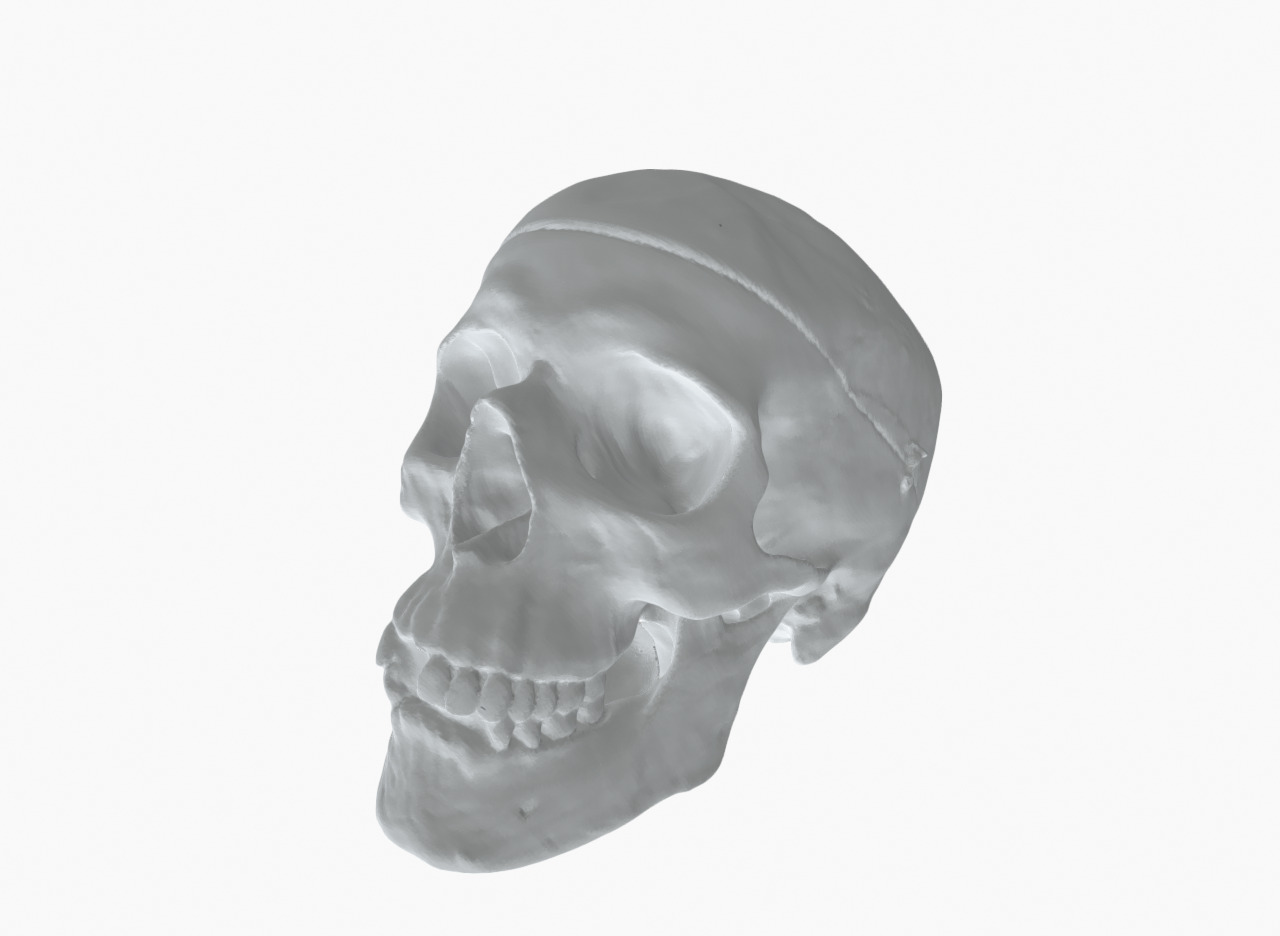
\includegraphics[width=0.2\textwidth]{images/chapter5_img/MeshReconResults/PositionalEncoding/65.jpg} & 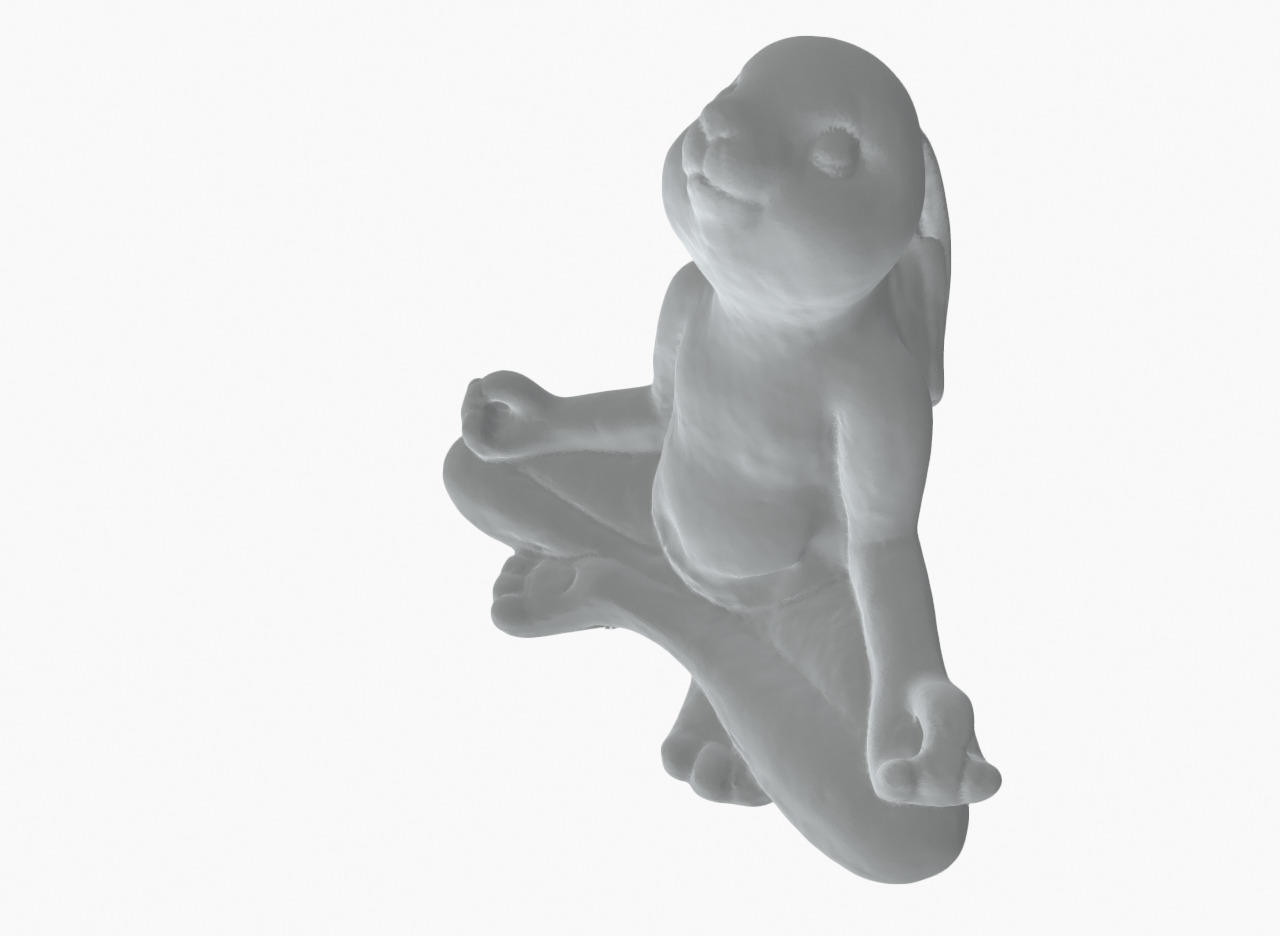
\includegraphics[width=0.2\textwidth]{images/chapter5_img/MeshReconResults/PositionalEncoding/110.jpg} & 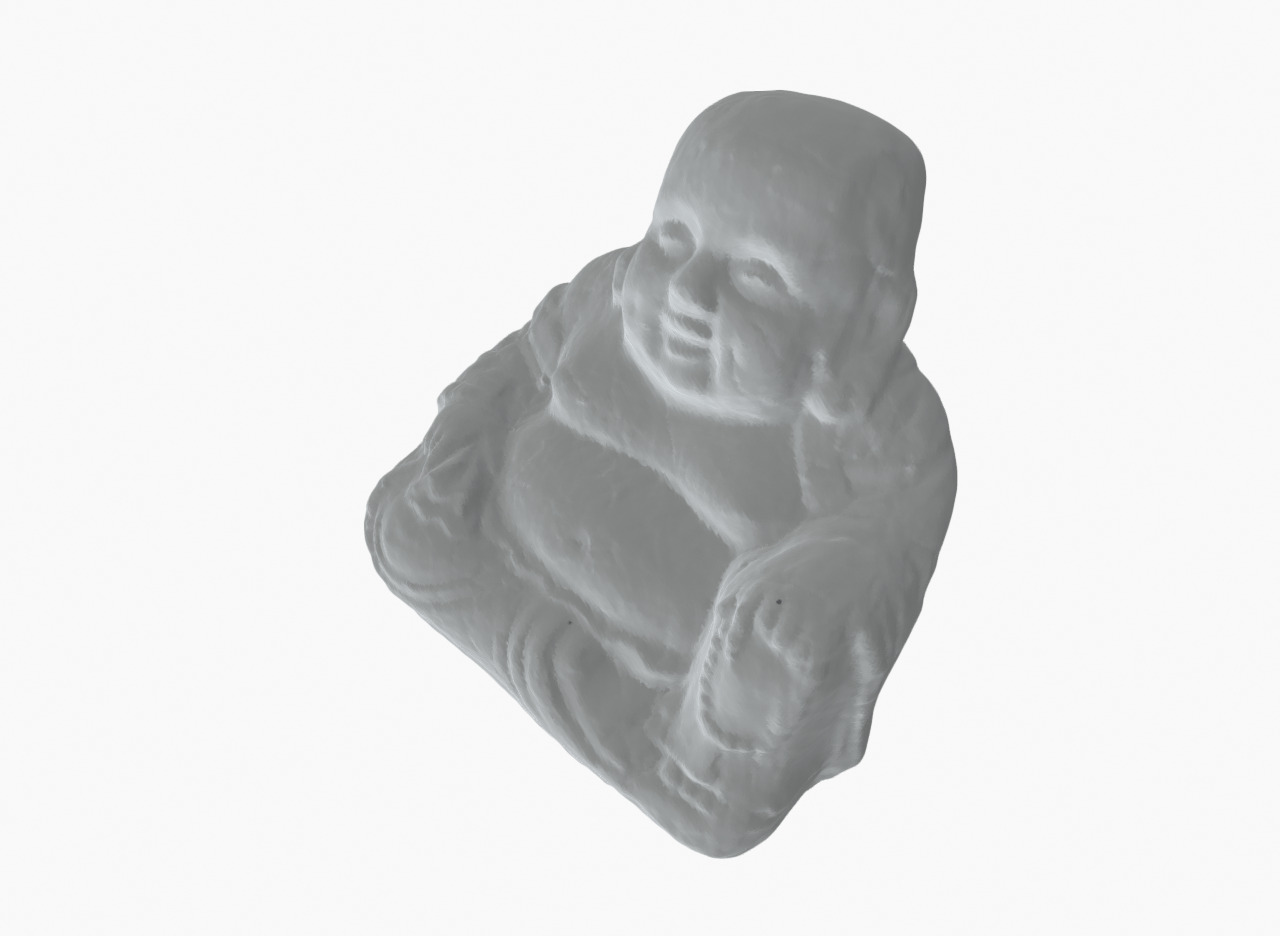
\includegraphics[width=0.2\textwidth]{images/chapter5_img/MeshReconResults/PositionalEncoding/114.jpg} & 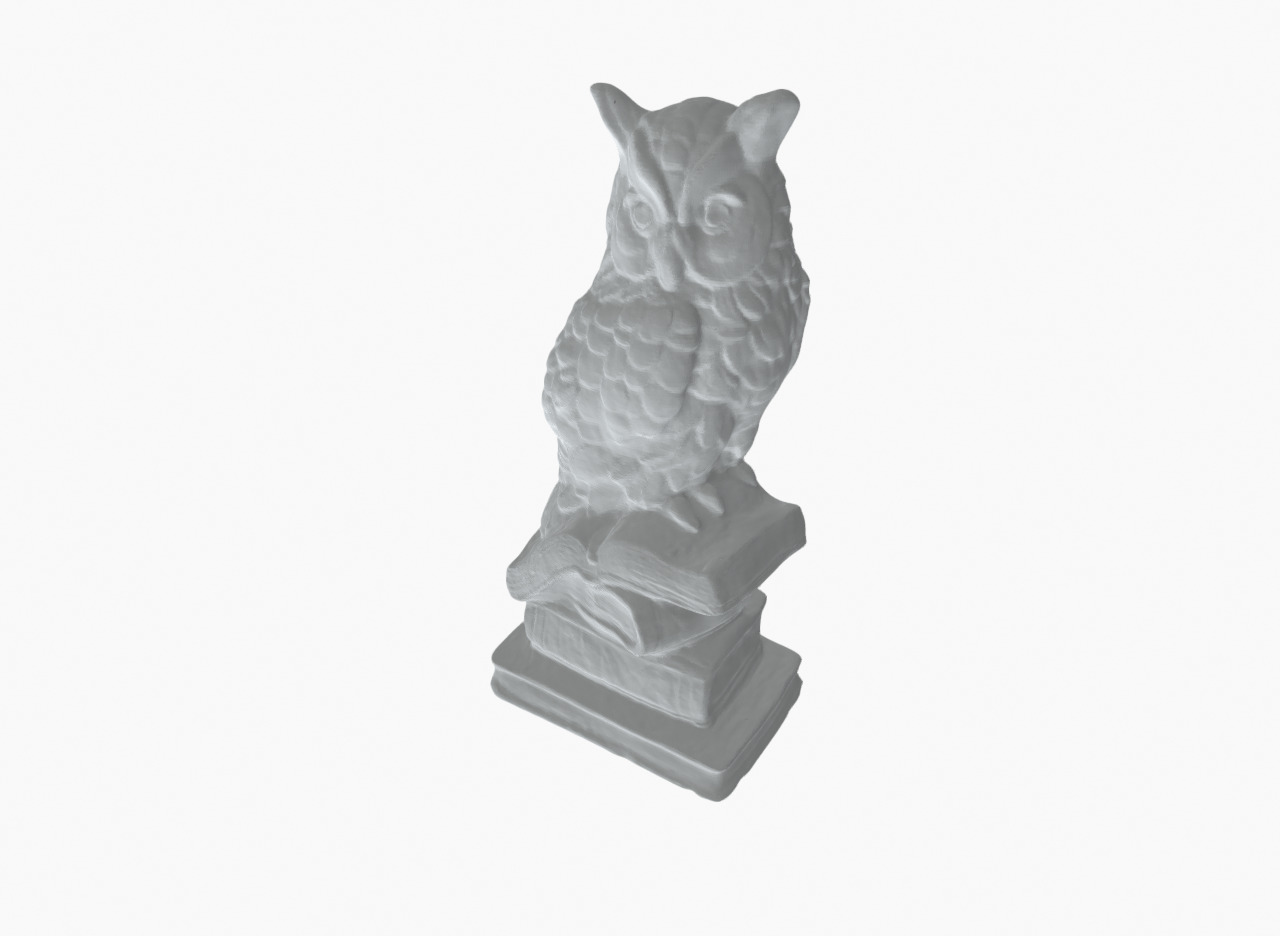
\includegraphics[width=0.2\textwidth]{images/chapter5_img/MeshReconResults/PositionalEncoding/122.jpg} \\
\hline
FourierNTK & 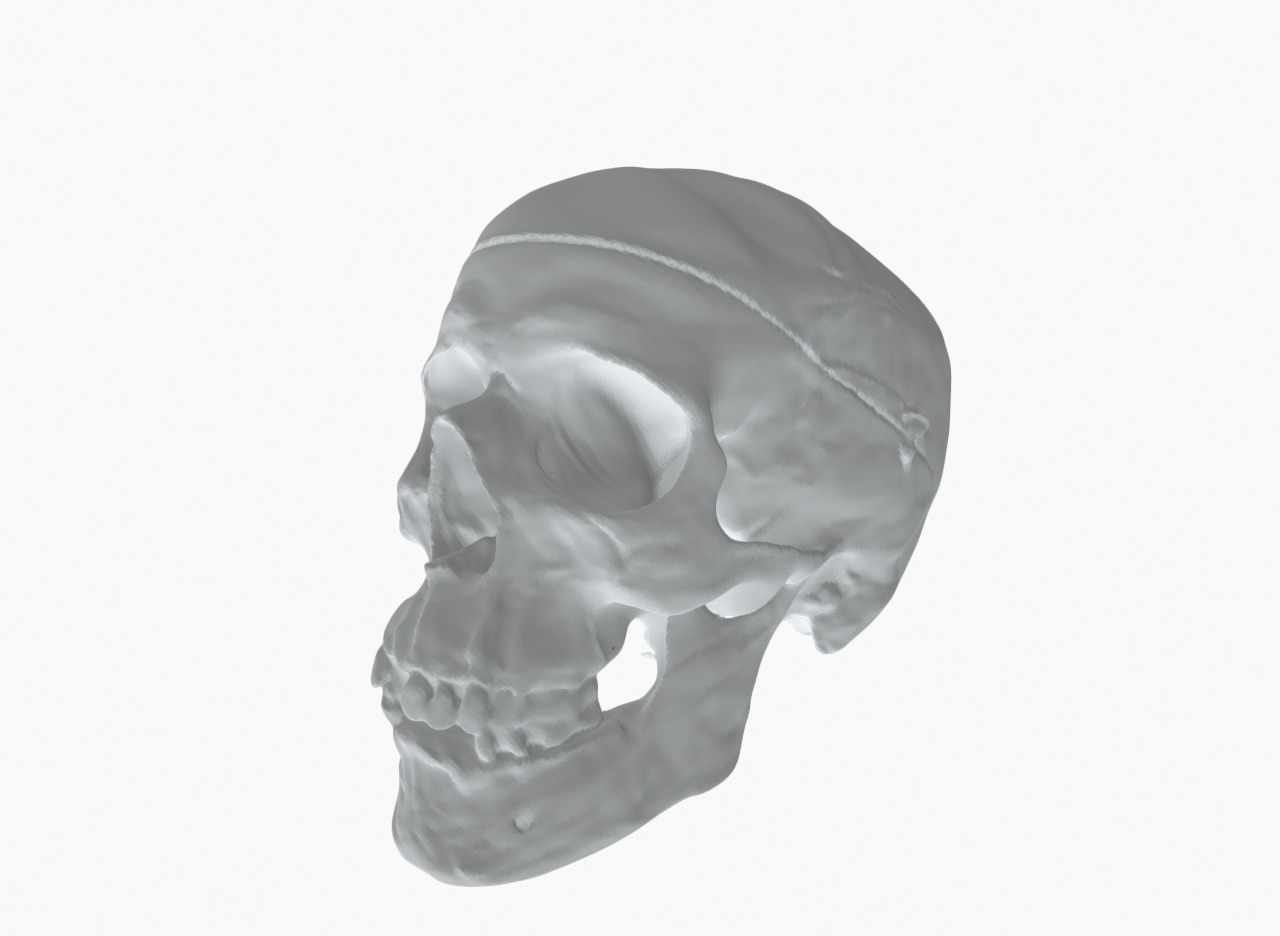
\includegraphics[width=0.2\textwidth]{images/chapter5_img/MeshReconResults/FourierNTK/65.jpg} & 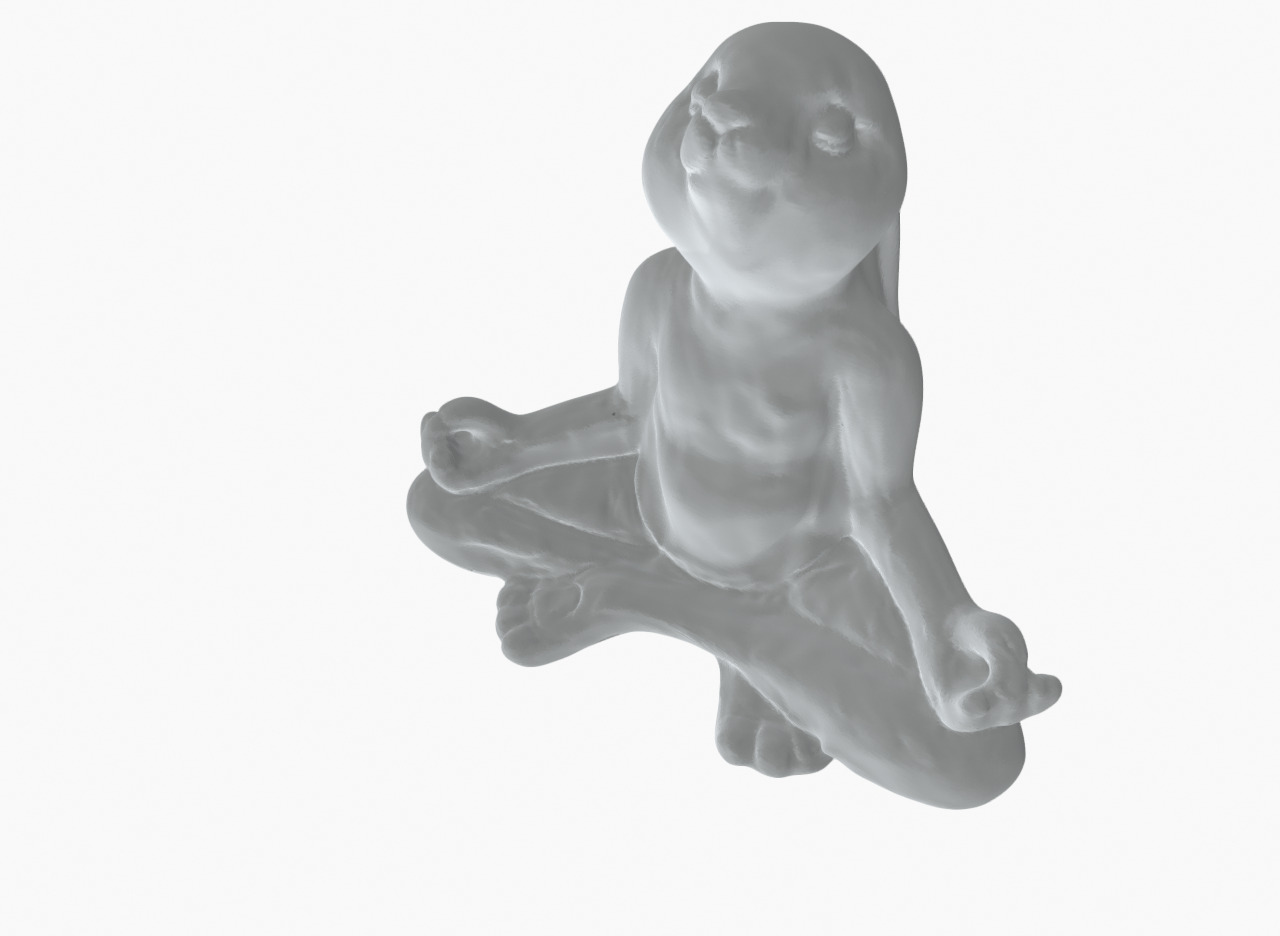
\includegraphics[width=0.2\textwidth]{images/chapter5_img/MeshReconResults/FourierNTK/110.jpg} & 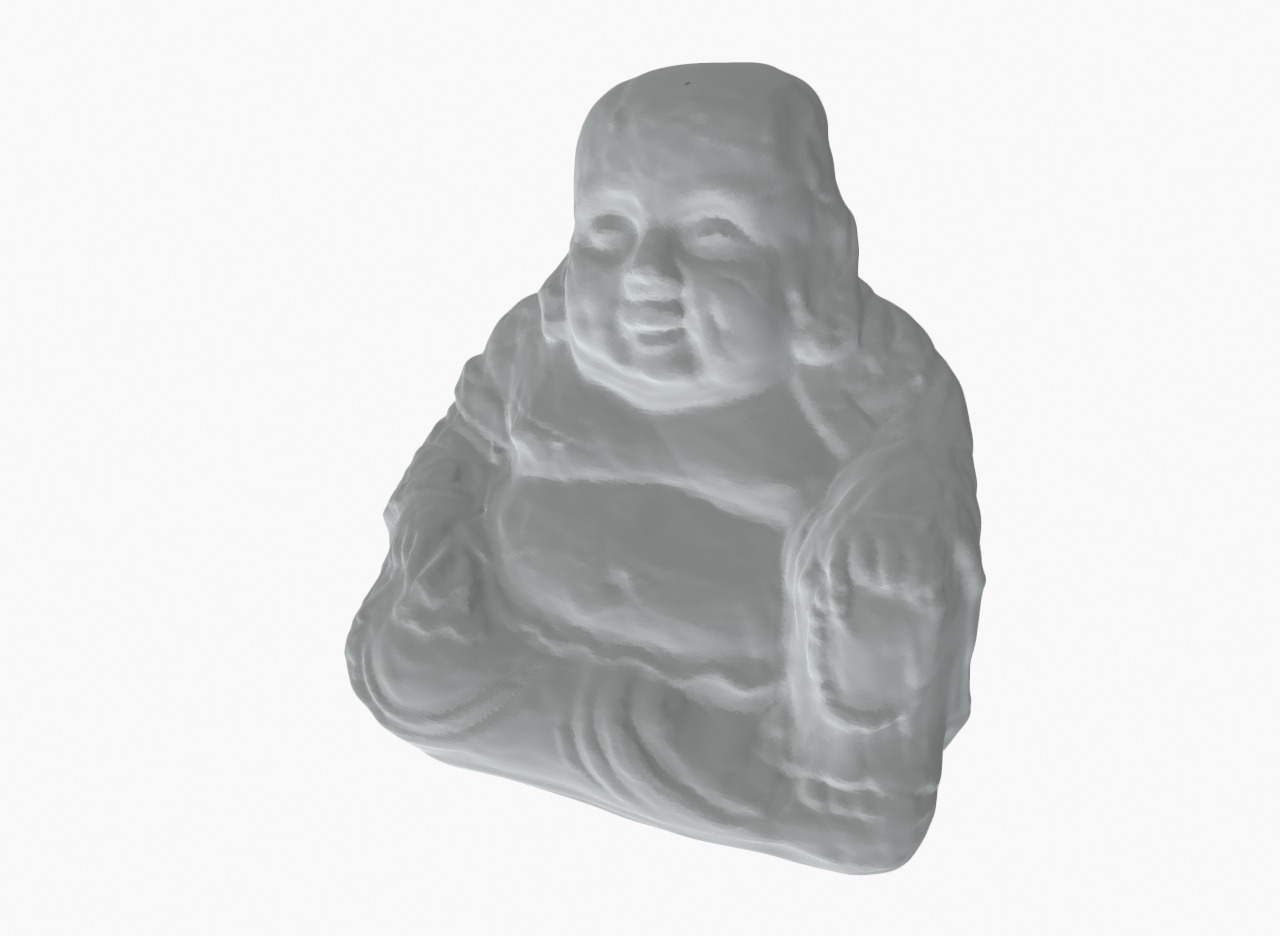
\includegraphics[width=0.2\textwidth]{images/chapter5_img/MeshReconResults/FourierNTK/114.jpg} & 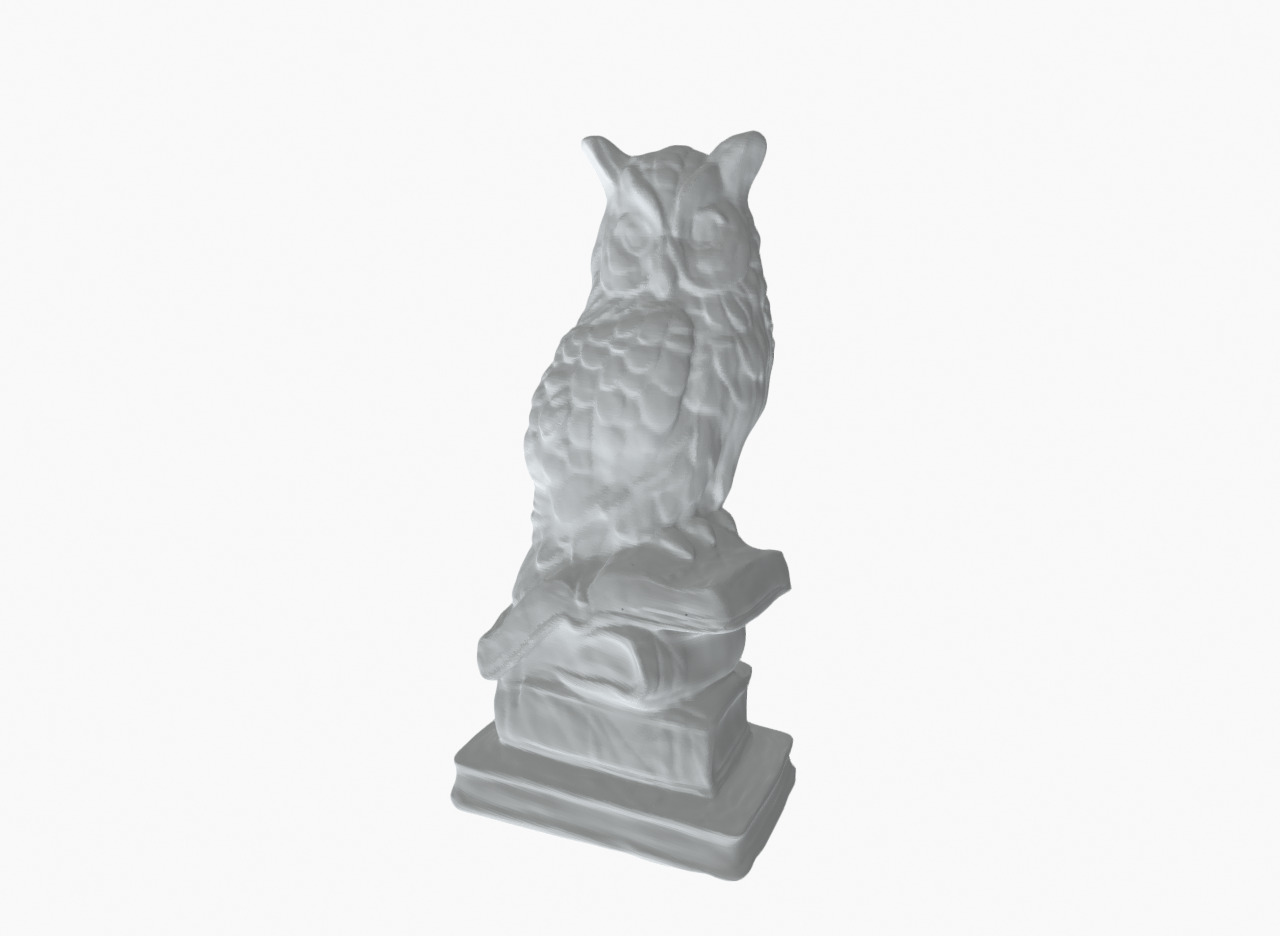
\includegraphics[width=0.2\textwidth]{images/chapter5_img/MeshReconResults/FourierNTK/122.jpg} \\
\hline
MR HashGrid3D & 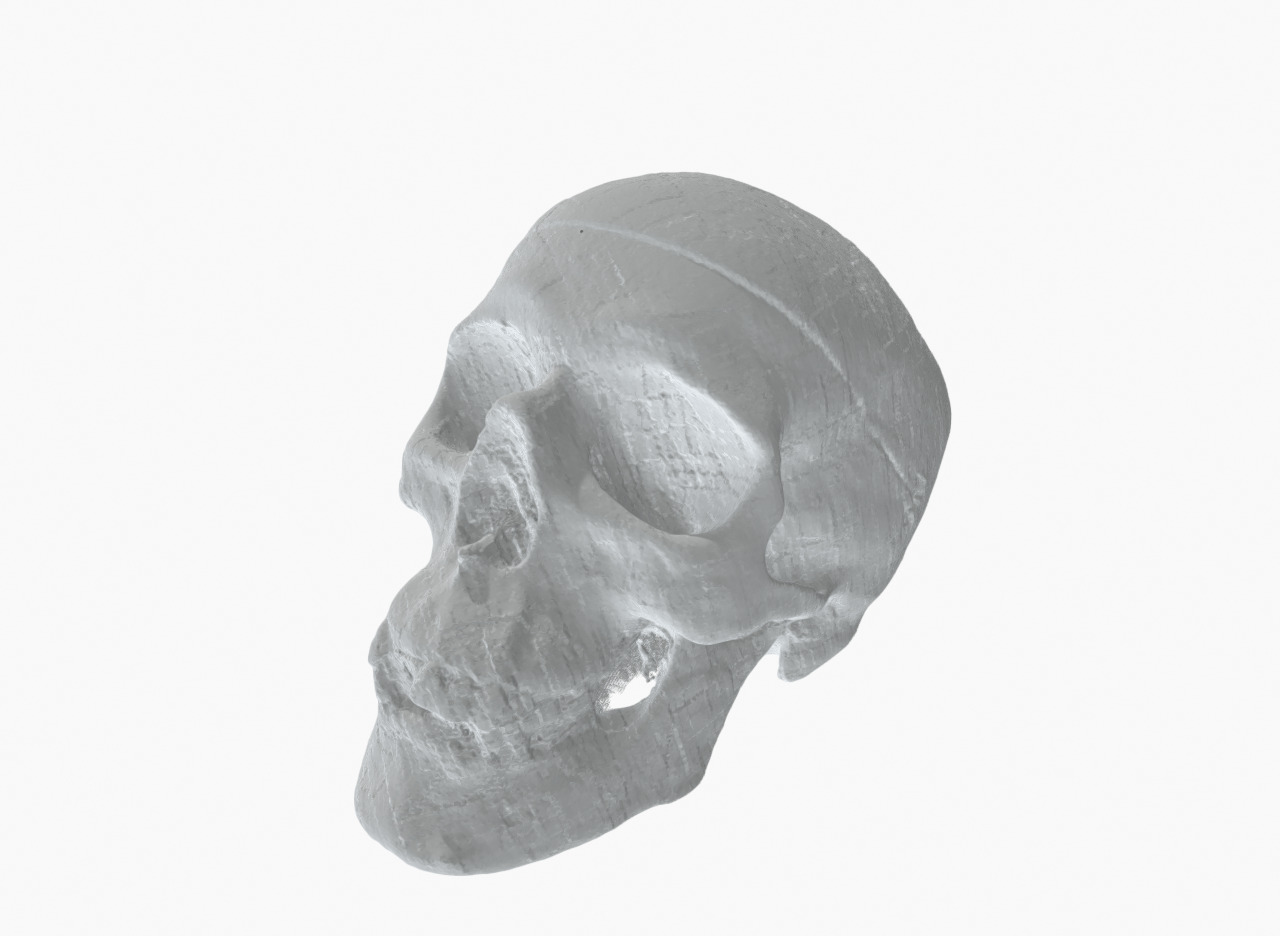
\includegraphics[width=0.2\textwidth]{images/chapter5_img/MeshReconResults/MRHashGrid3D/65.jpg} & 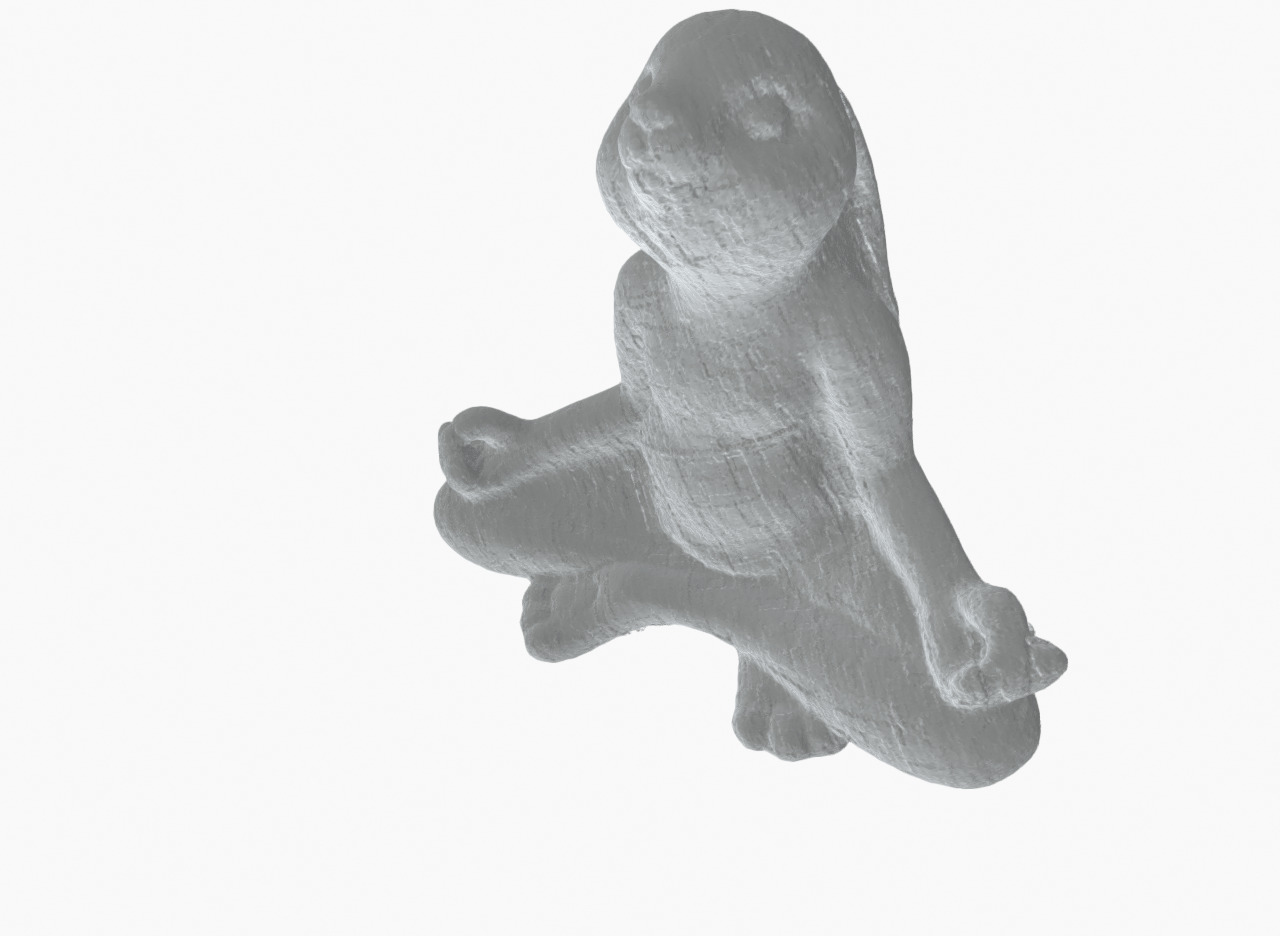
\includegraphics[width=0.2\textwidth]{images/chapter5_img/MeshReconResults/MRHashGrid3D/110.jpg} & 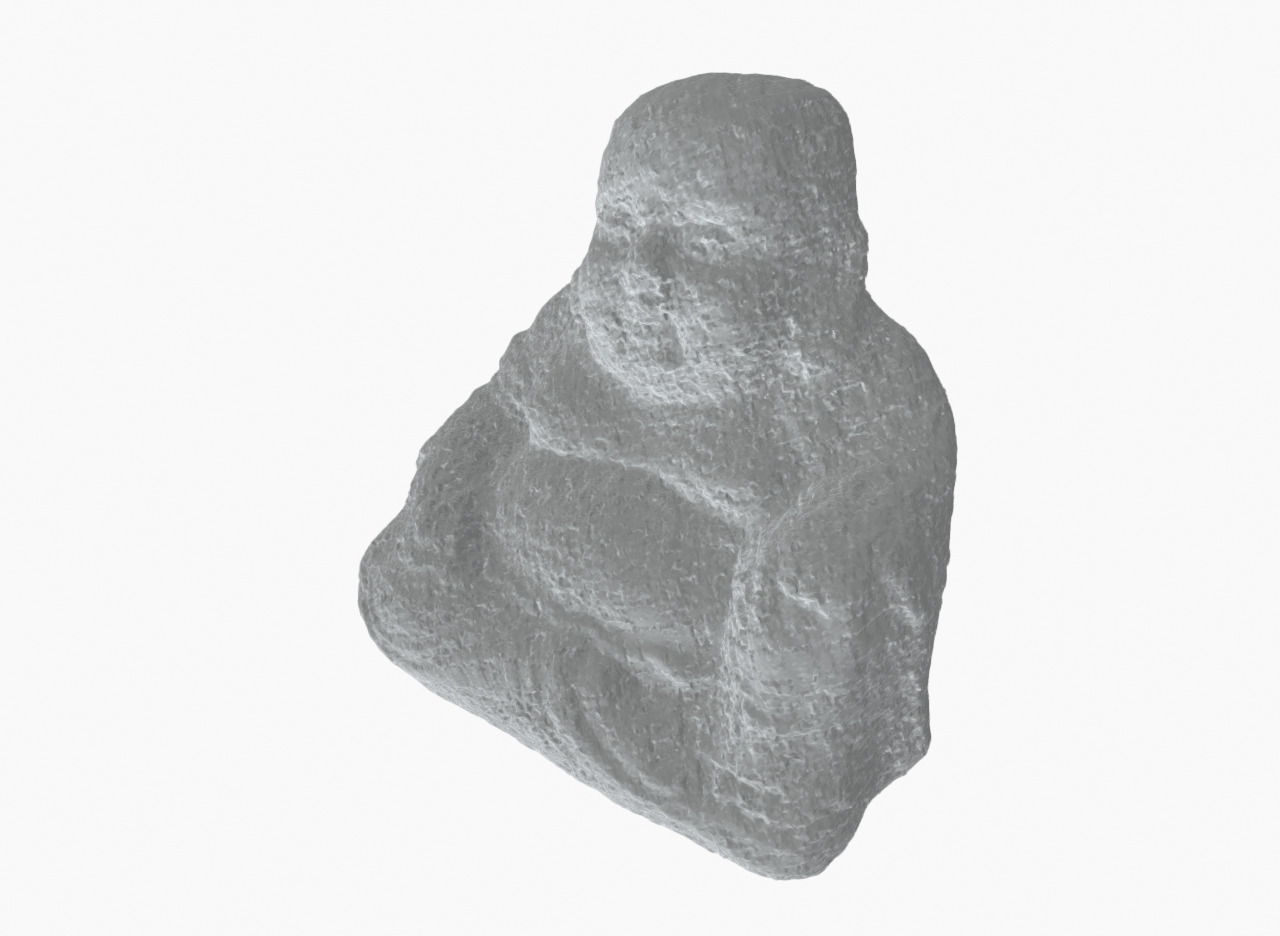
\includegraphics[width=0.2\textwidth]{images/chapter5_img/MeshReconResults/MRHashGrid3D/114.jpg} & 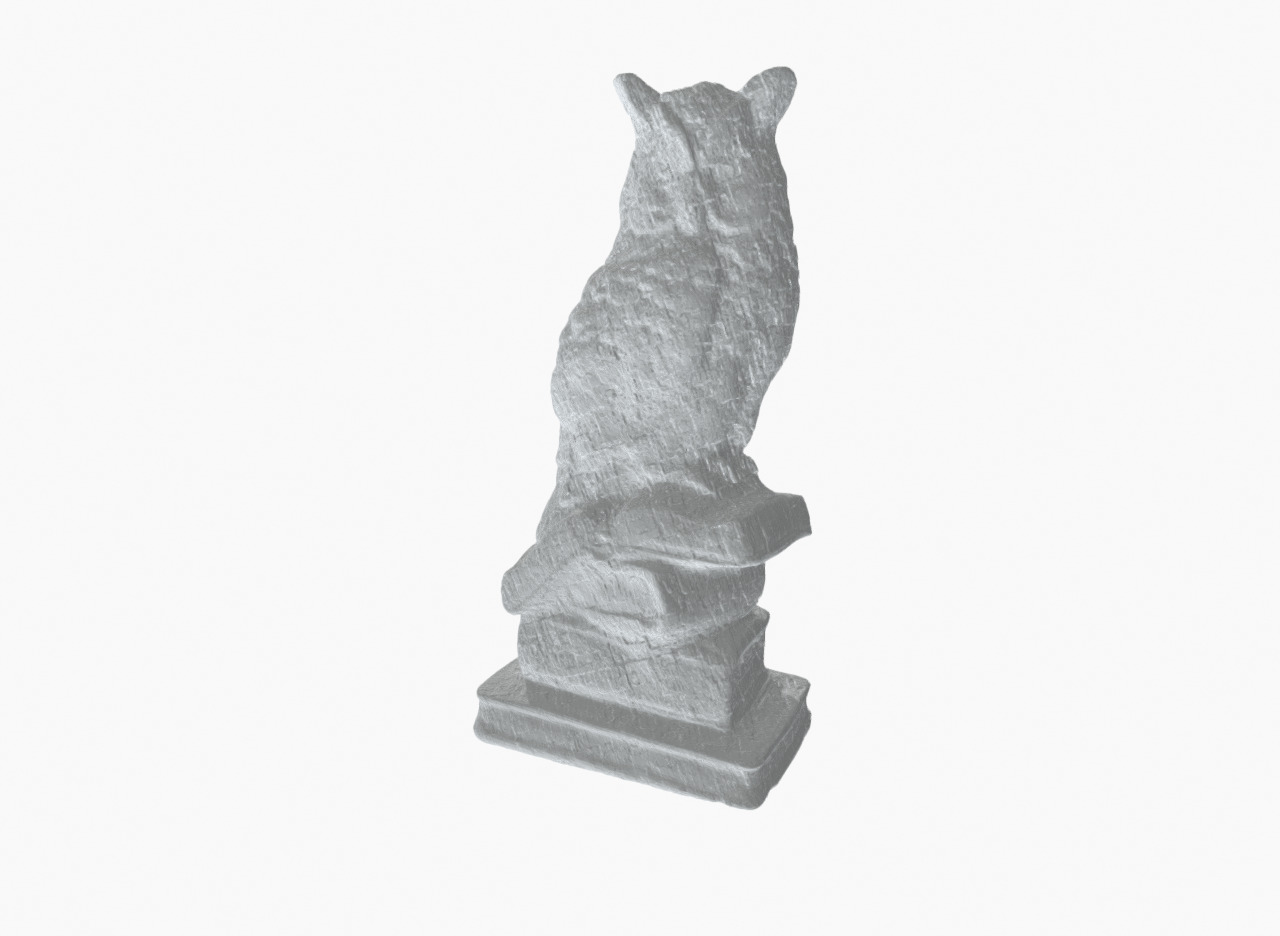
\includegraphics[width=0.2\textwidth]{images/chapter5_img/MeshReconResults/MRHashGrid3D/122.jpg} \\
\hline
NFFB & 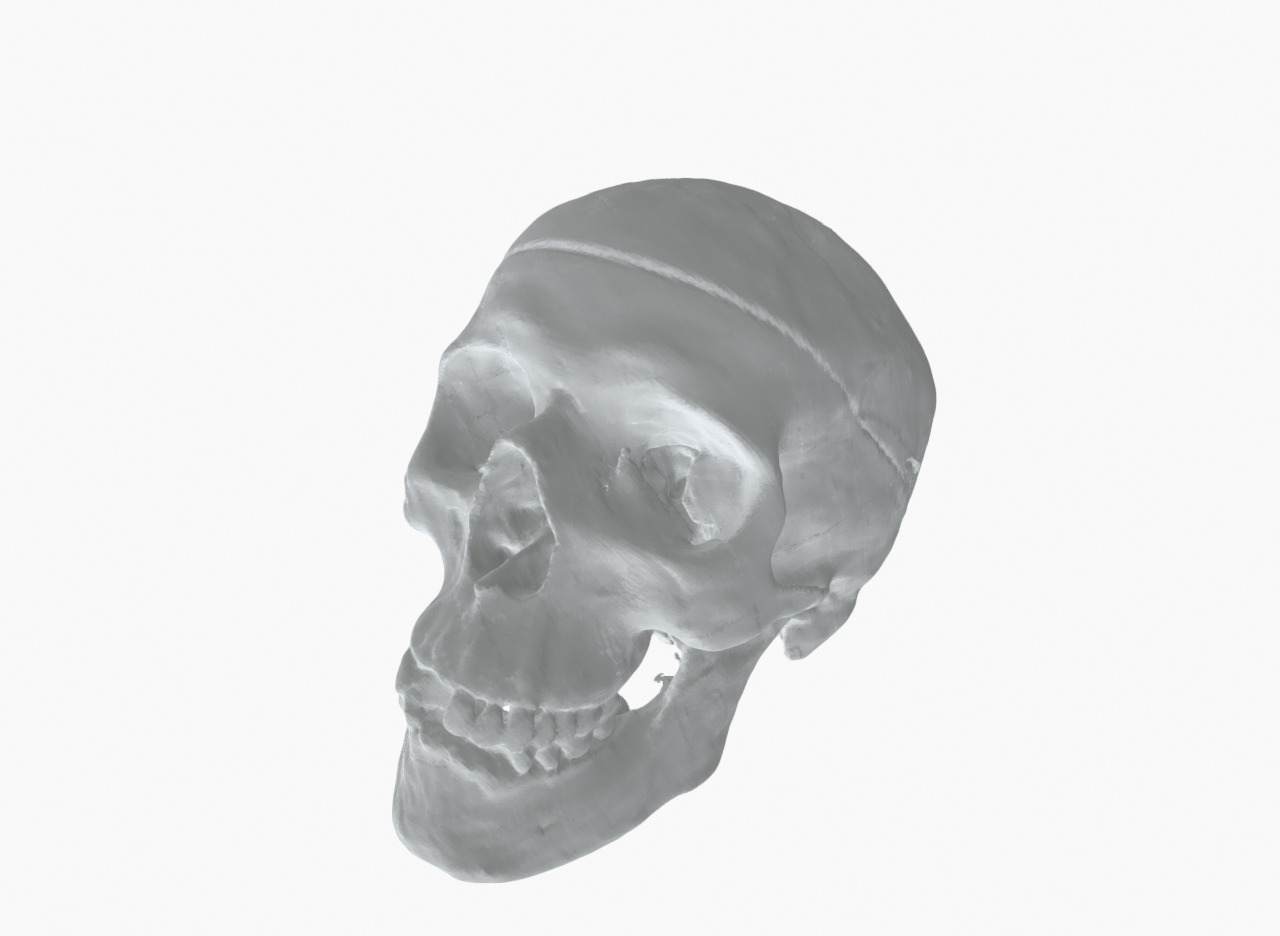
\includegraphics[width=0.2\textwidth]{images/chapter5_img/MeshReconResults/NFFB/65.jpg} & 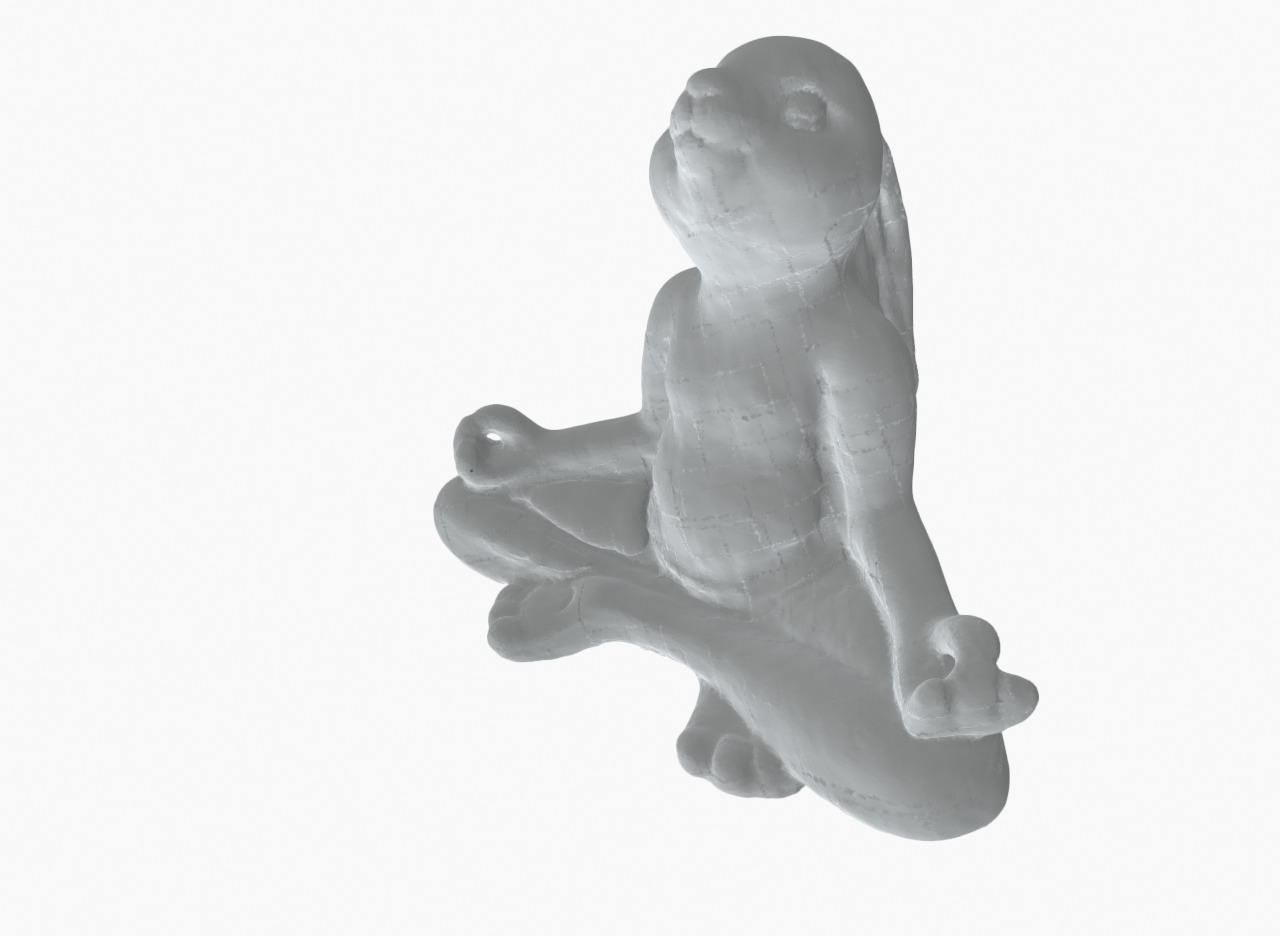
\includegraphics[width=0.2\textwidth]{images/chapter5_img/MeshReconResults/NFFB/110.jpg} & 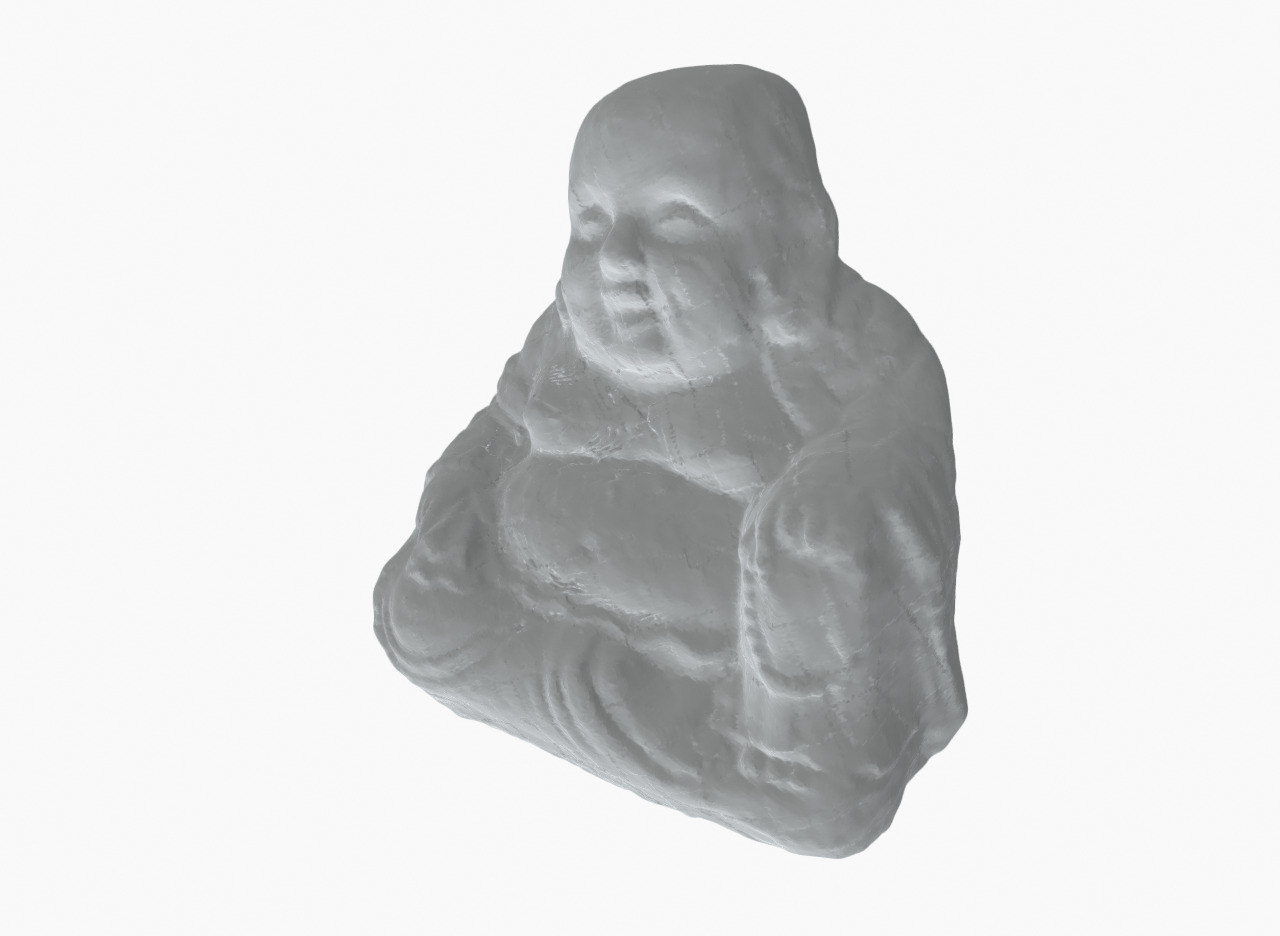
\includegraphics[width=0.2\textwidth]{images/chapter5_img/MeshReconResults/NFFB/114.jpg} & 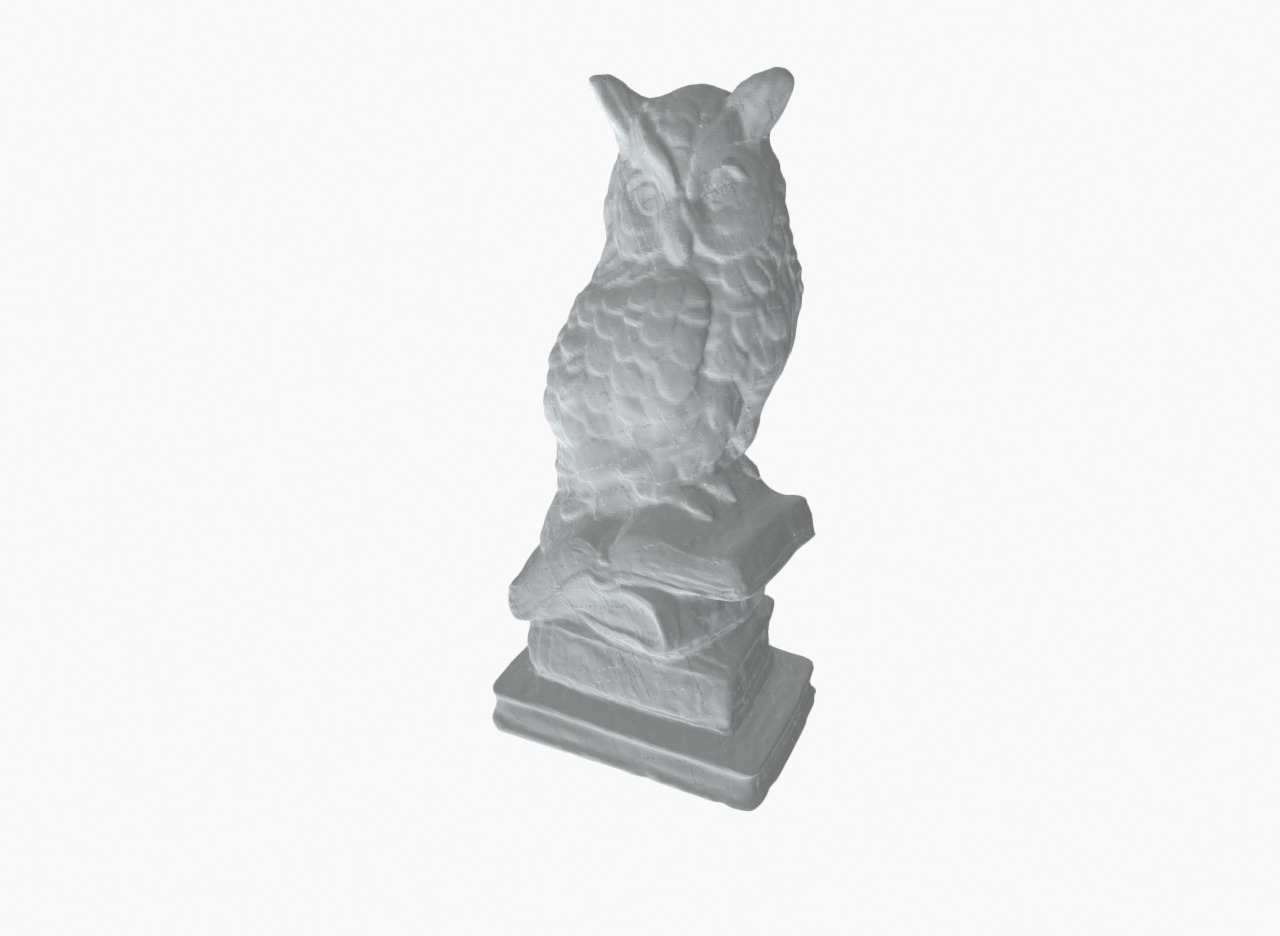
\includegraphics[width=0.2\textwidth]{images/chapter5_img/MeshReconResults/NFFB/122.jpg} \\
\hline
Stylemod NFFB & 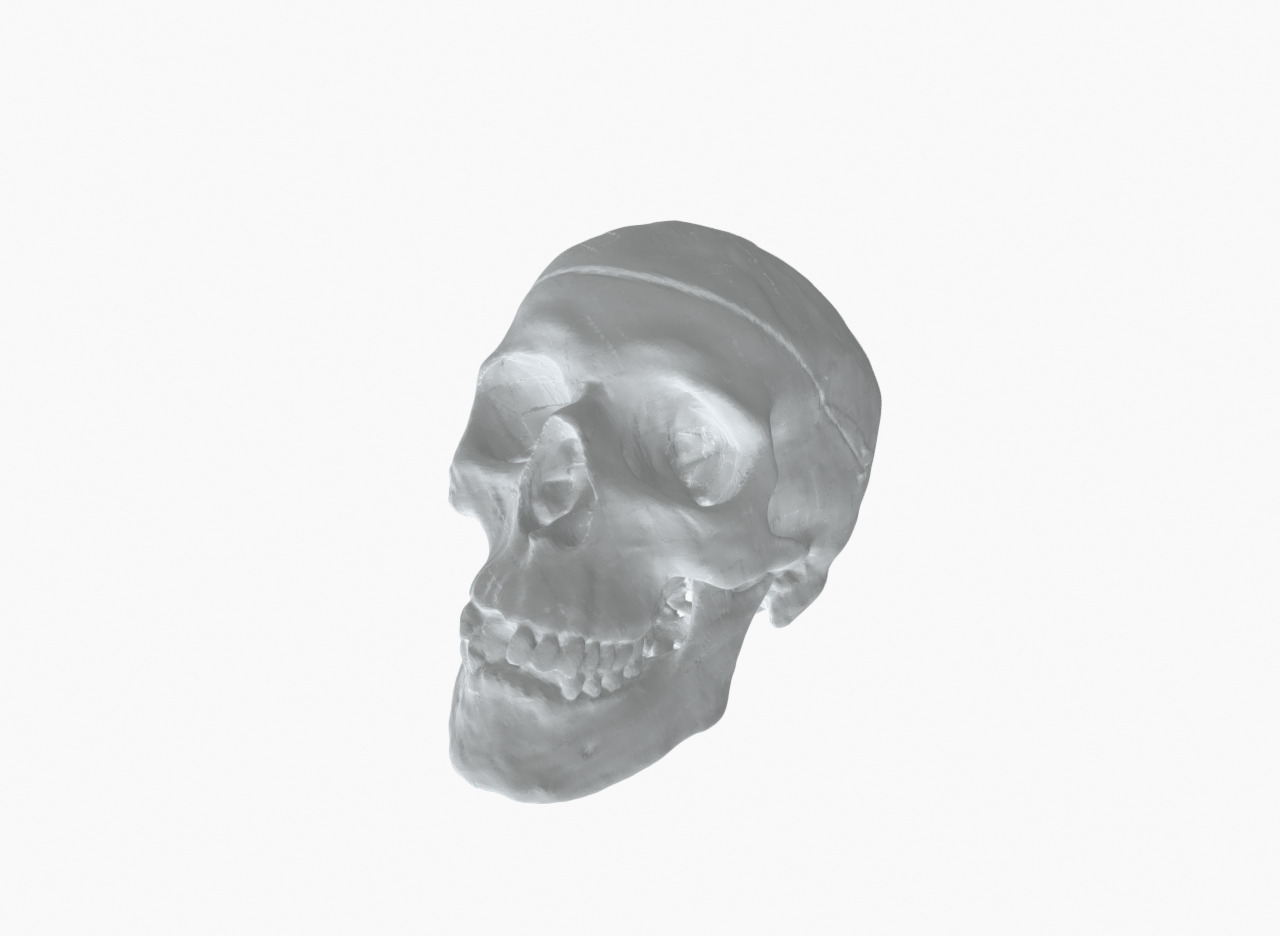
\includegraphics[width=0.2\textwidth]{images/chapter5_img/MeshReconResults/StylemodNFFB/65.jpg} & 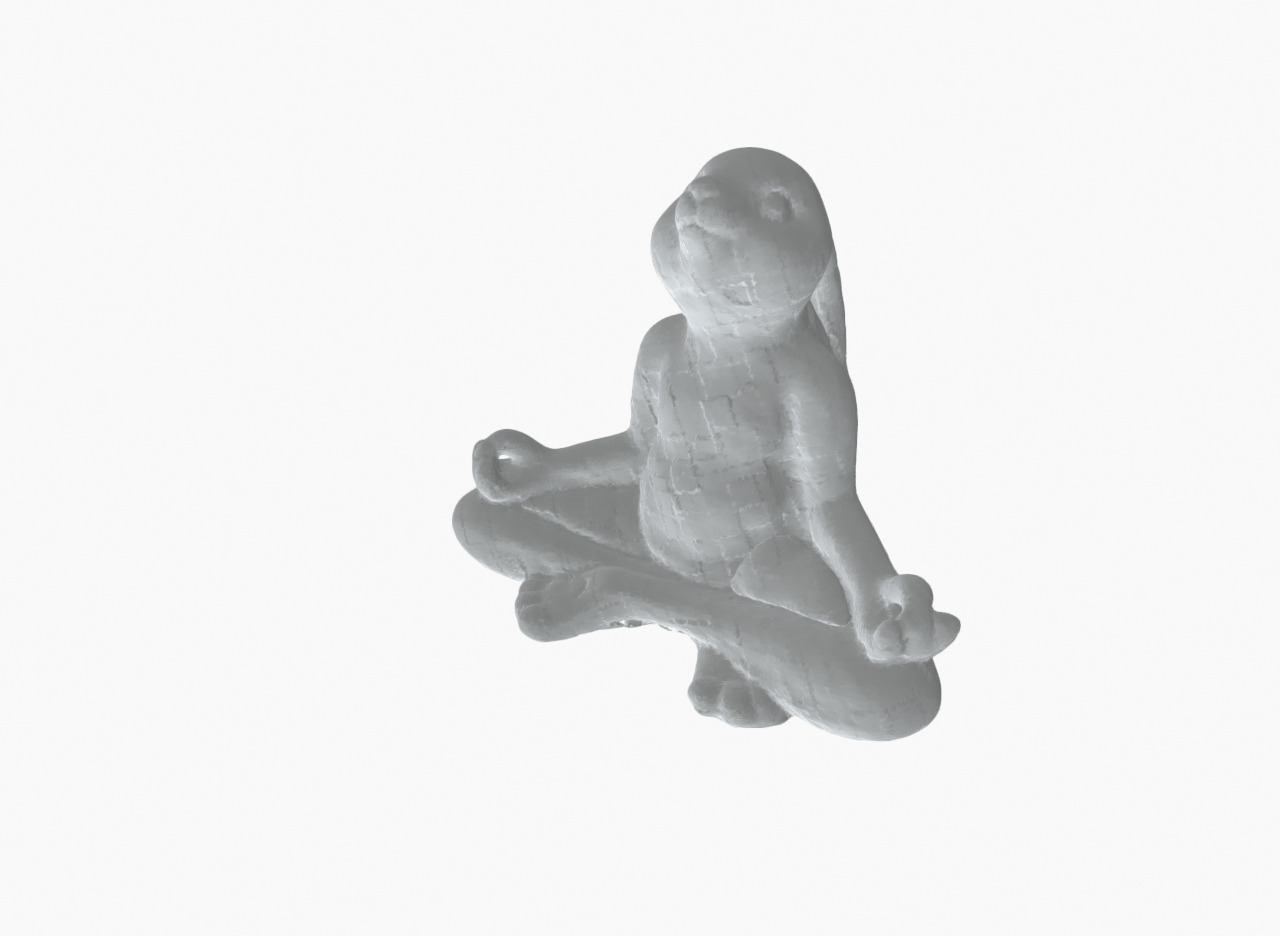
\includegraphics[width=0.2\textwidth]{images/chapter5_img/MeshReconResults/StylemodNFFB/110.jpg} & 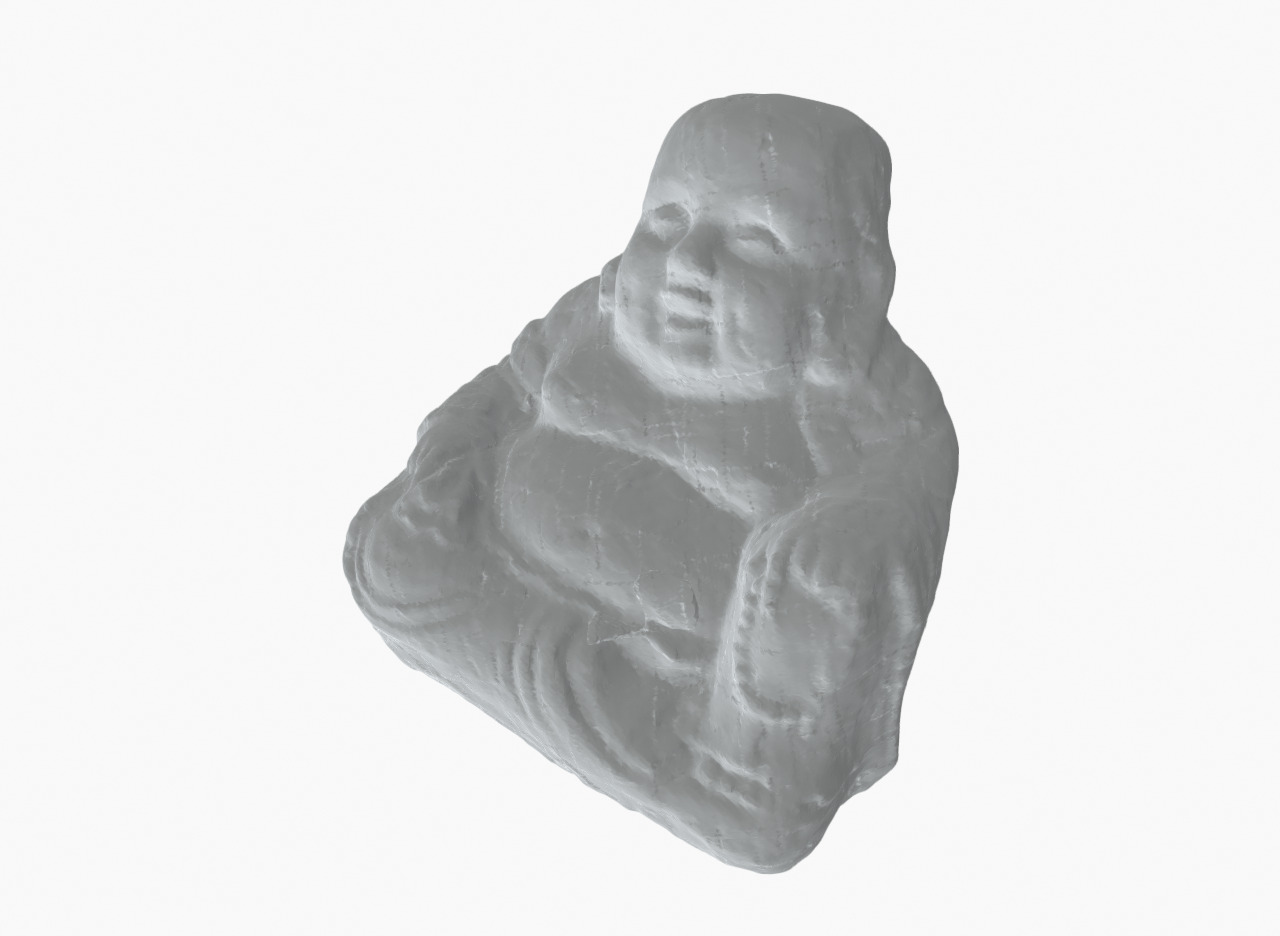
\includegraphics[width=0.2\textwidth]{images/chapter5_img/MeshReconResults/StylemodNFFB/114.jpg} & 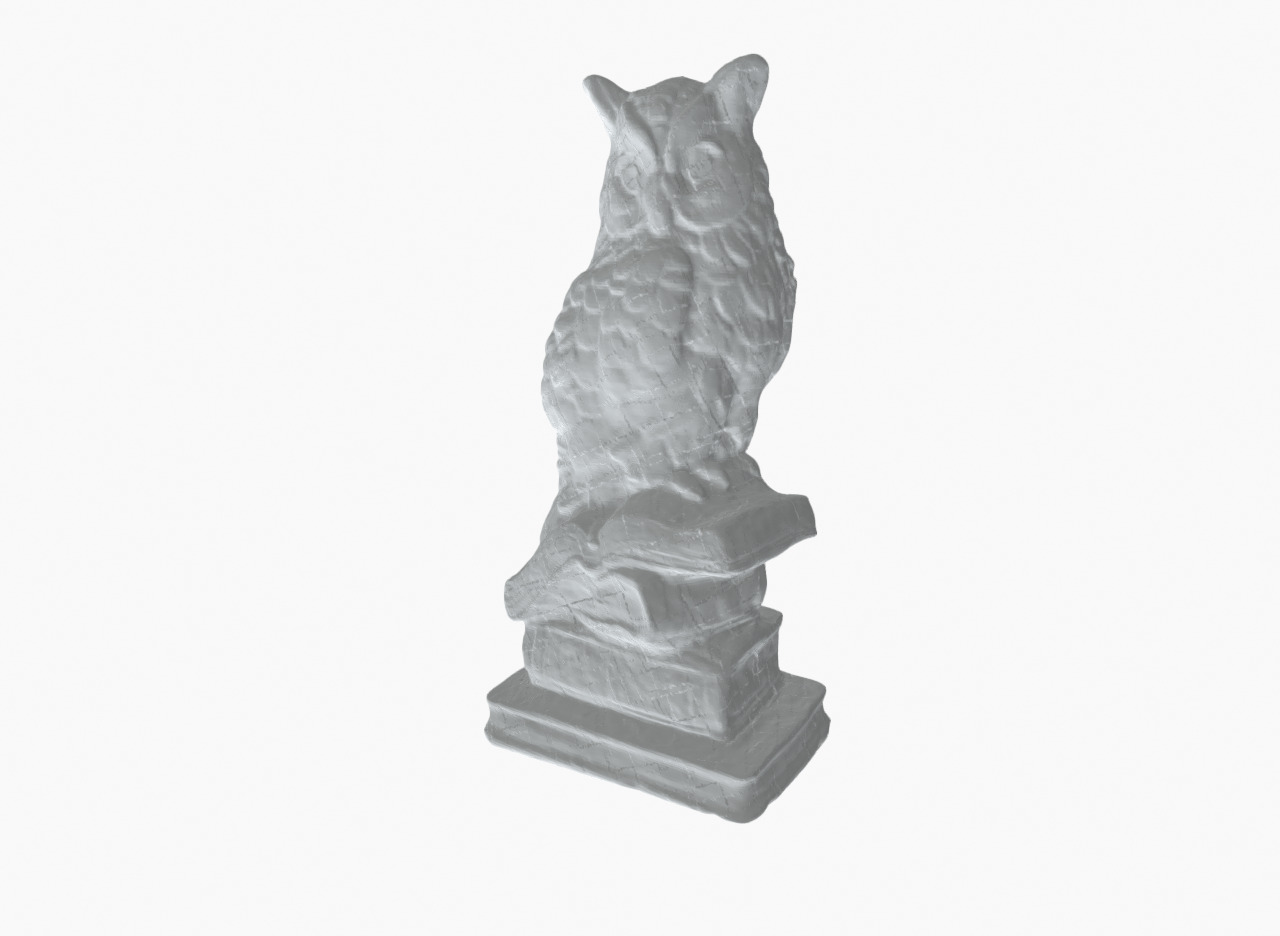
\includegraphics[width=0.2\textwidth]{images/chapter5_img/MeshReconResults/StylemodNFFB/122.jpg} \\
\hline
Stylemod NFFB TCNN & 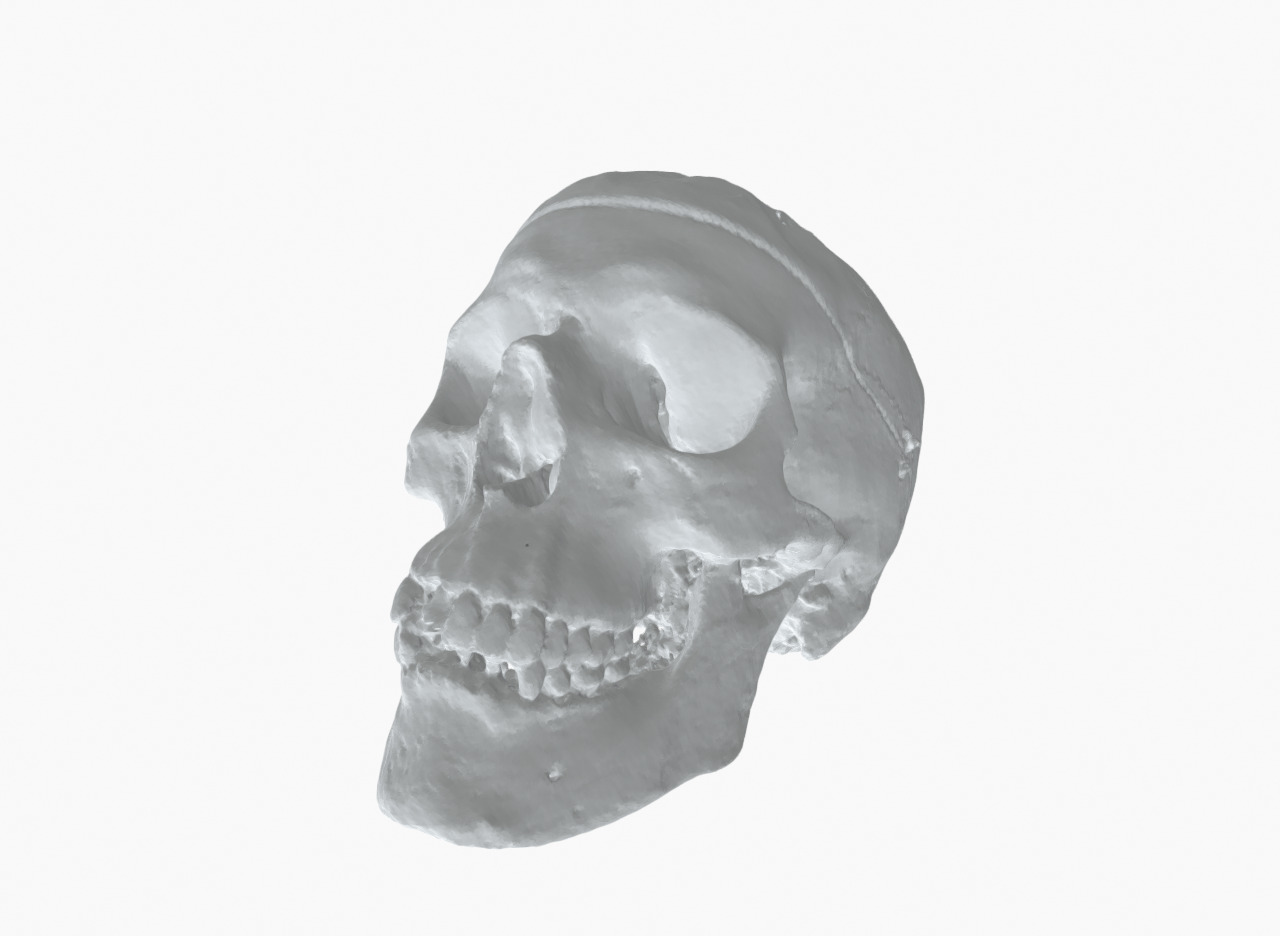
\includegraphics[width=0.2\textwidth]{images/chapter5_img/MeshReconResults/TinyCudaNN-StylemodNFFB/65_2000.jpg} & 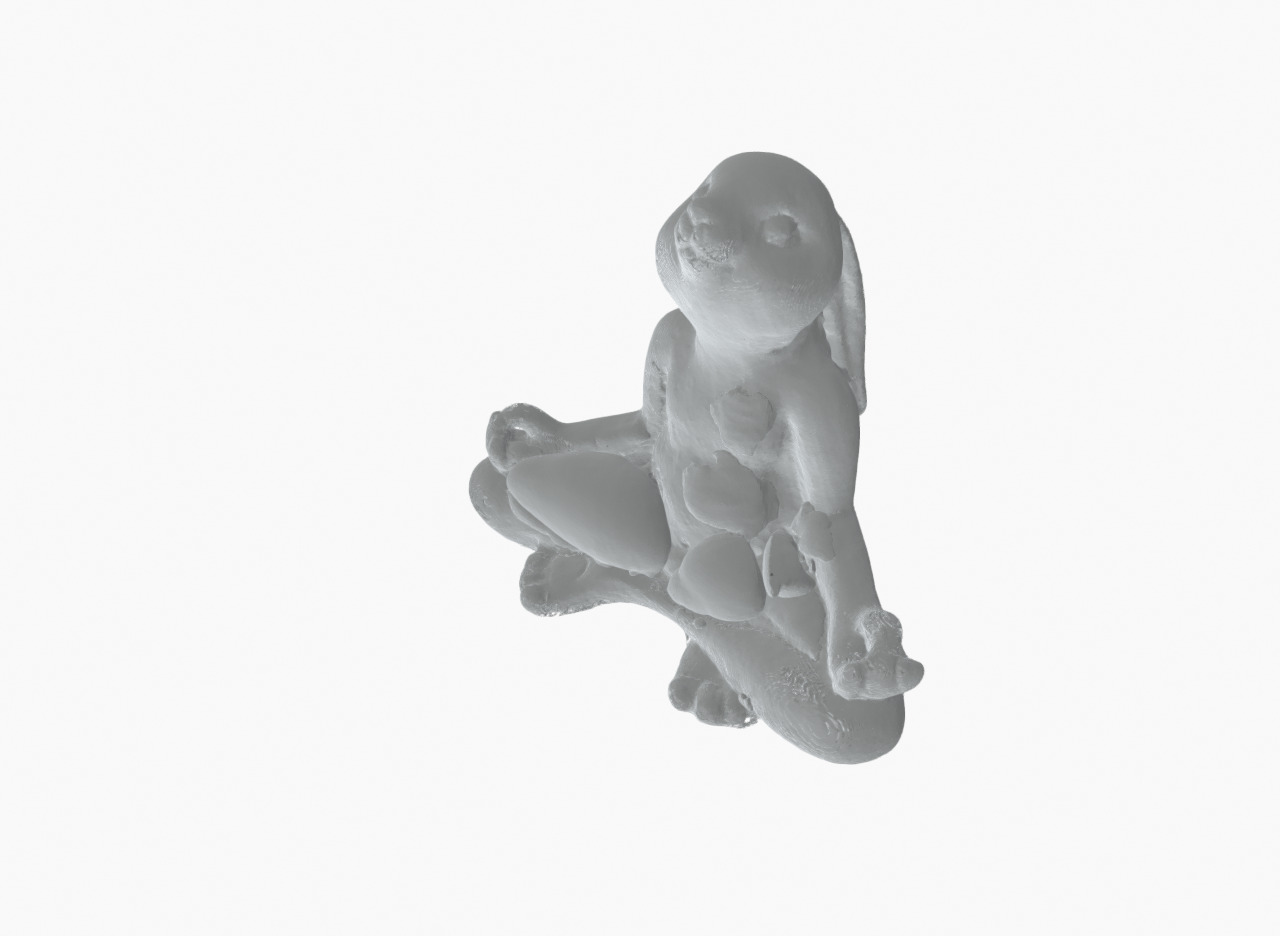
\includegraphics[width=0.2\textwidth]{images/chapter5_img/MeshReconResults/TinyCudaNN-StylemodNFFB/110_bad.jpg} & 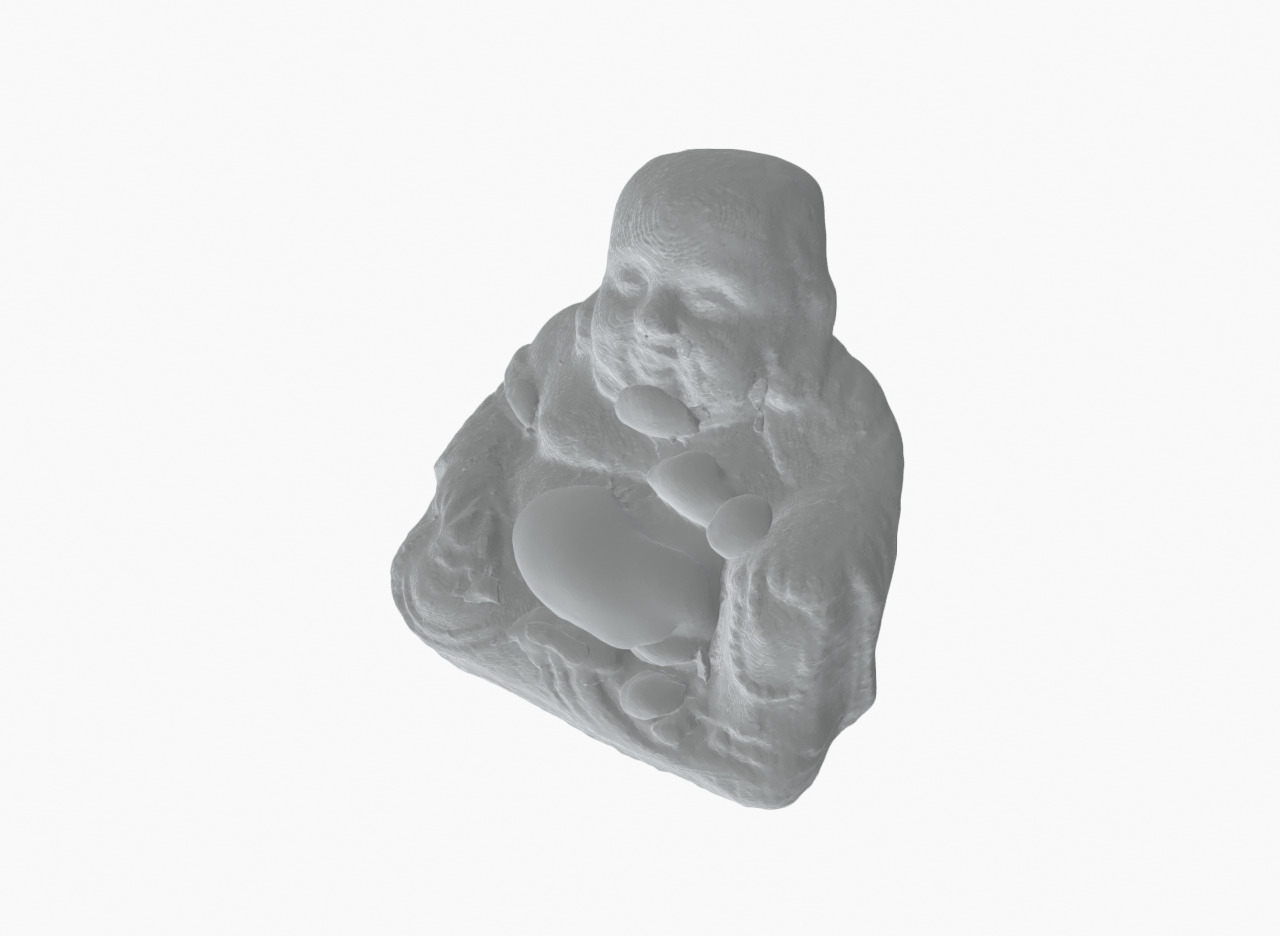
\includegraphics[width=0.2\textwidth]{images/chapter5_img/MeshReconResults/TinyCudaNN-StylemodNFFB/114_2000.jpg} & 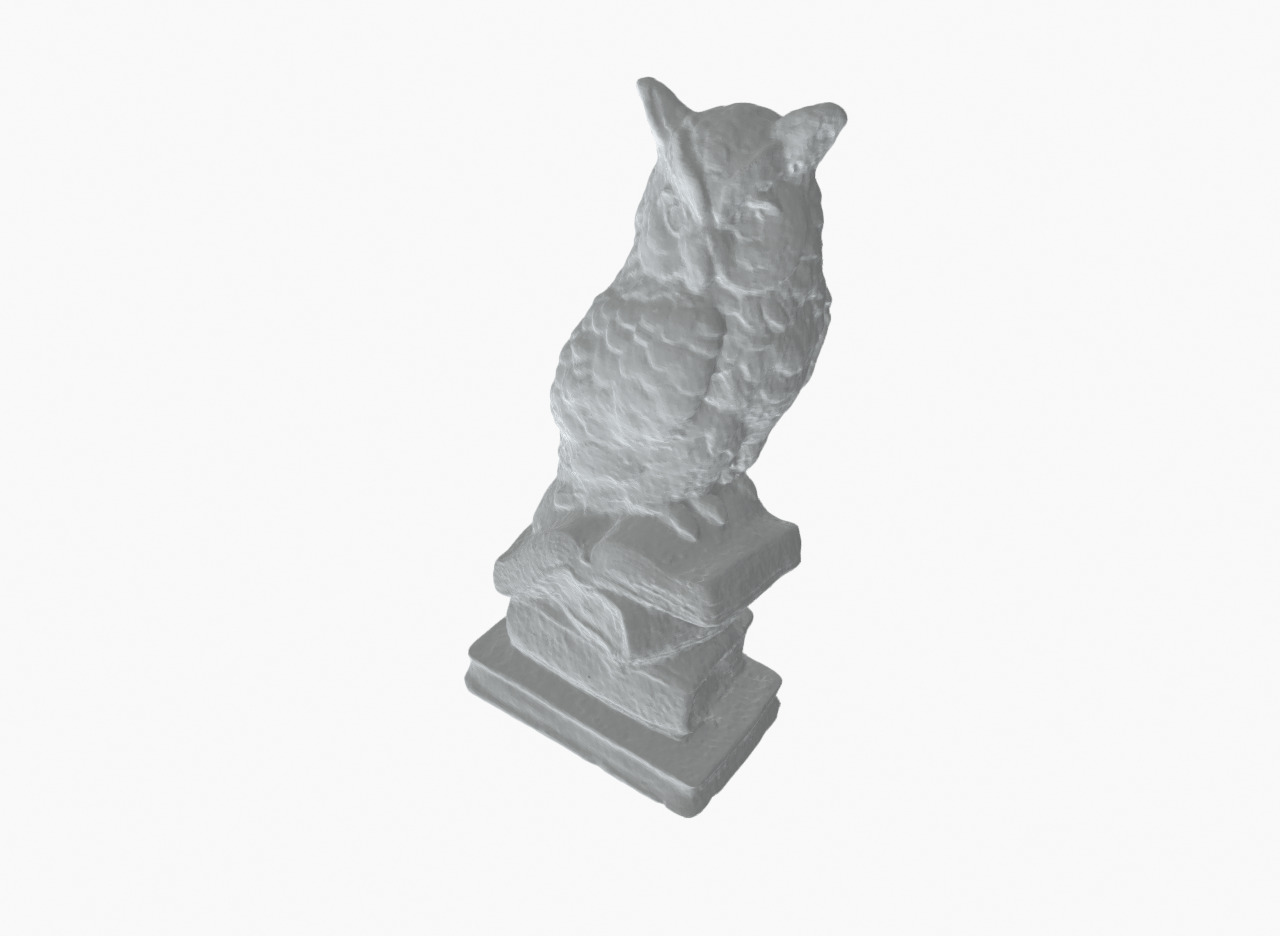
\includegraphics[width=0.2\textwidth]{images/chapter5_img/MeshReconResults/TinyCudaNN-StylemodNFFB/122.jpg} \\
\hline
HashGrid3D TCNN & & 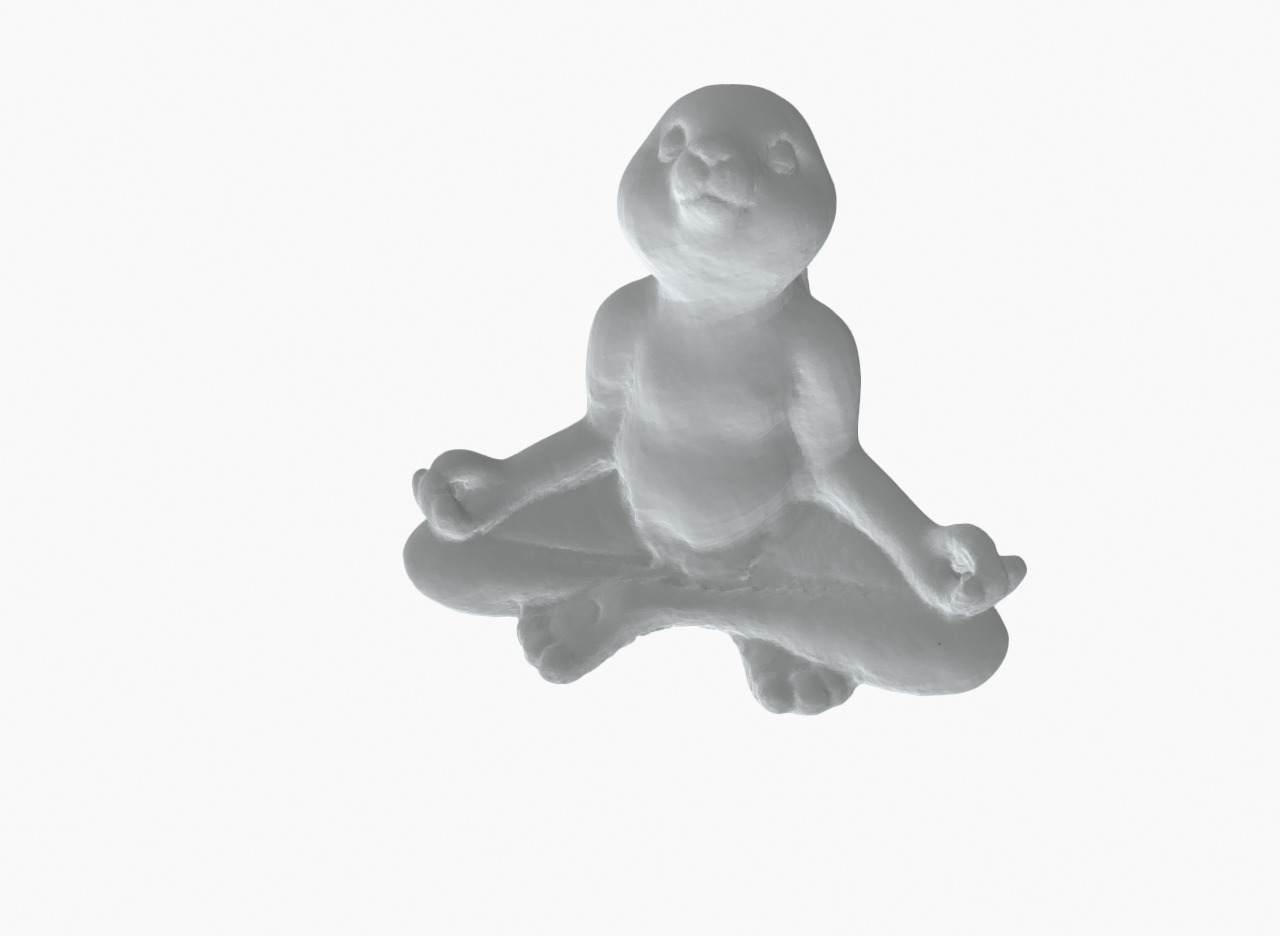
\includegraphics[width=0.2\textwidth]{images/chapter5_img/MeshReconResults/TinyCUDANN-MRHashGrid3D/110.jpg} & & 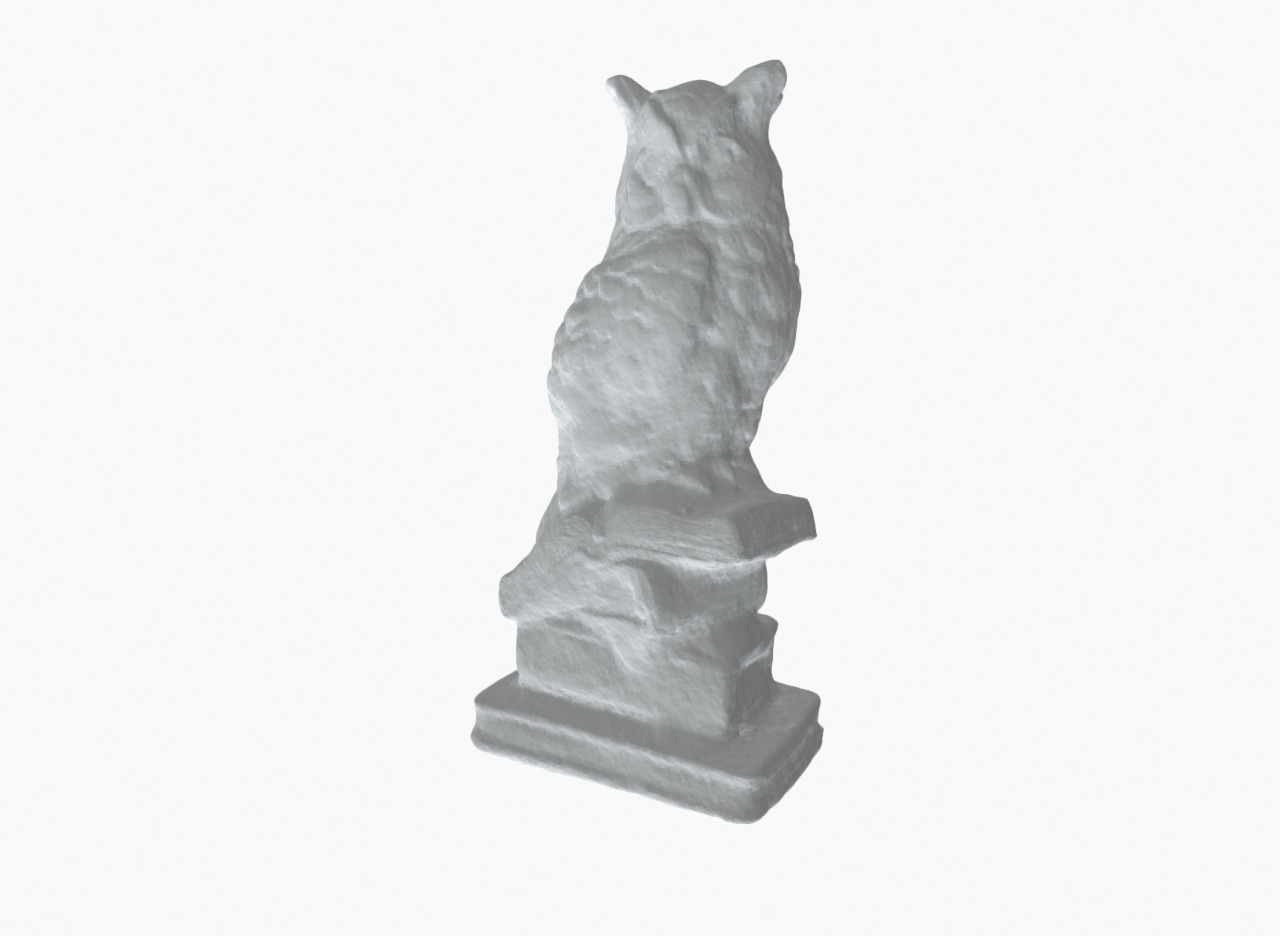
\includegraphics[width=0.2\textwidth]{images/chapter5_img/MeshReconResults/TinyCUDANN-MRHashGrid3D/122.jpg} \\
\hline
\end{tabularx}
\caption{Πίνακας Γεωμετρίας \enit{3D} μοντέλων}
\end{table}
\clearpage
Ενδιαφέρον παρουσιάζει και η κρυφή όψη:
\begin{table}[H]
\begin{tabularx}{\textwidth}{|p{3.2cm}|X|X|X|X|}
\hline
Algorithm Name & Scan 65 & Scan 110 & Scan 114 & Scan 122 \\
\hline
Positional Encoding & 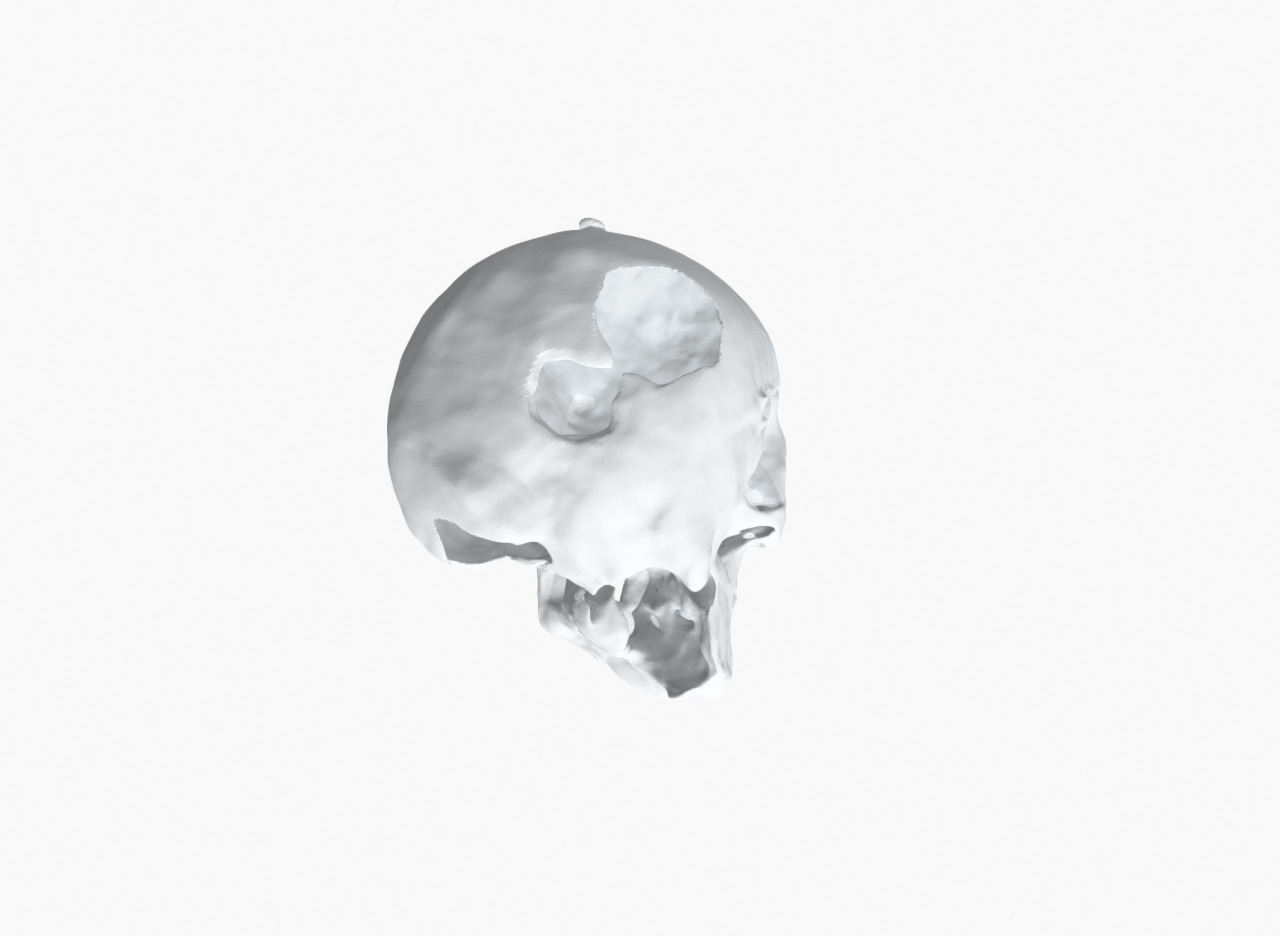
\includegraphics[width=0.2\textwidth]{images/chapter5_img/MeshReconResults/PositionalEncoding/65-HiddenView.jpg} & 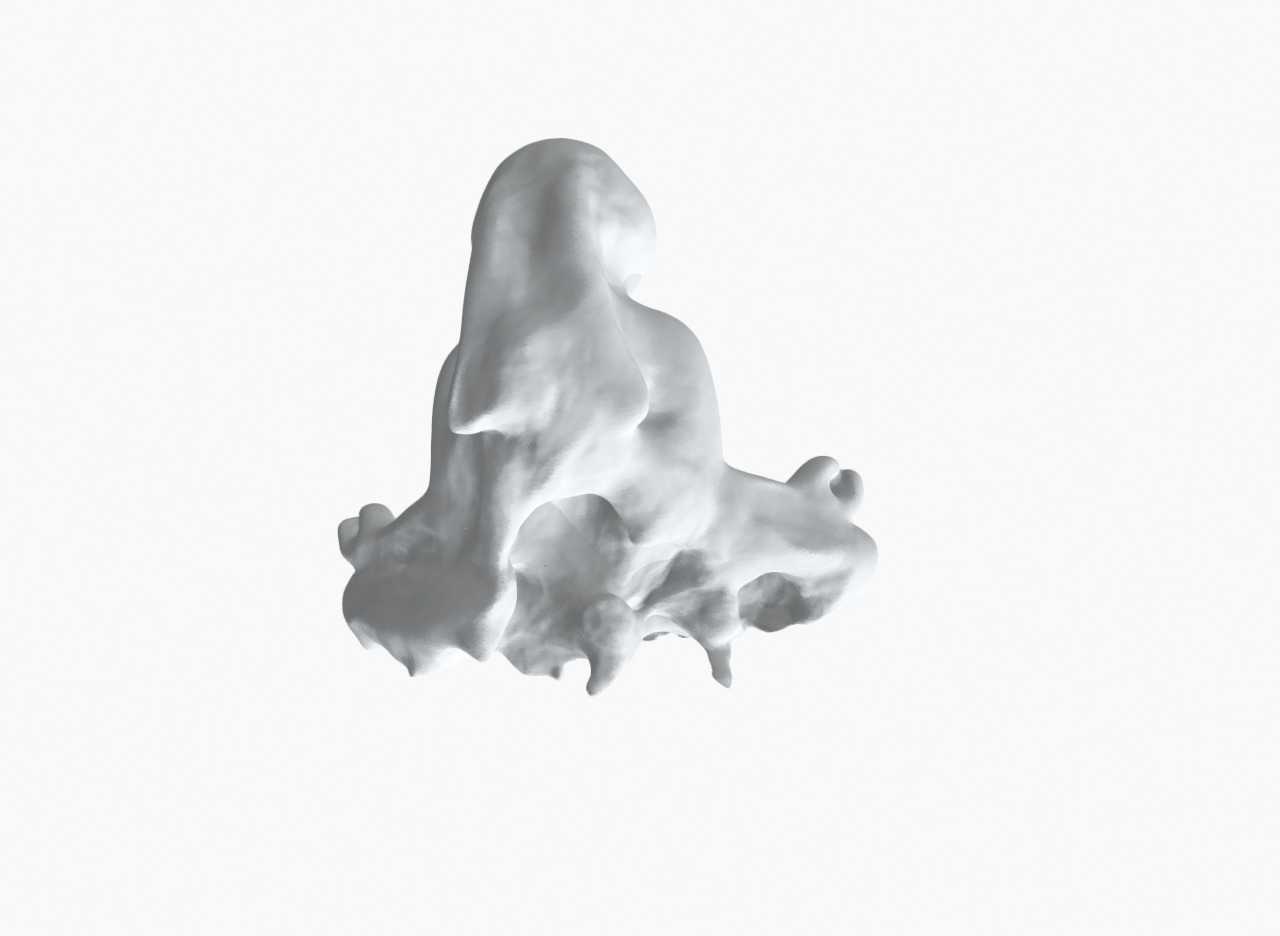
\includegraphics[width=0.2\textwidth]{images/chapter5_img/MeshReconResults/PositionalEncoding/110-HiddenView.jpg} & 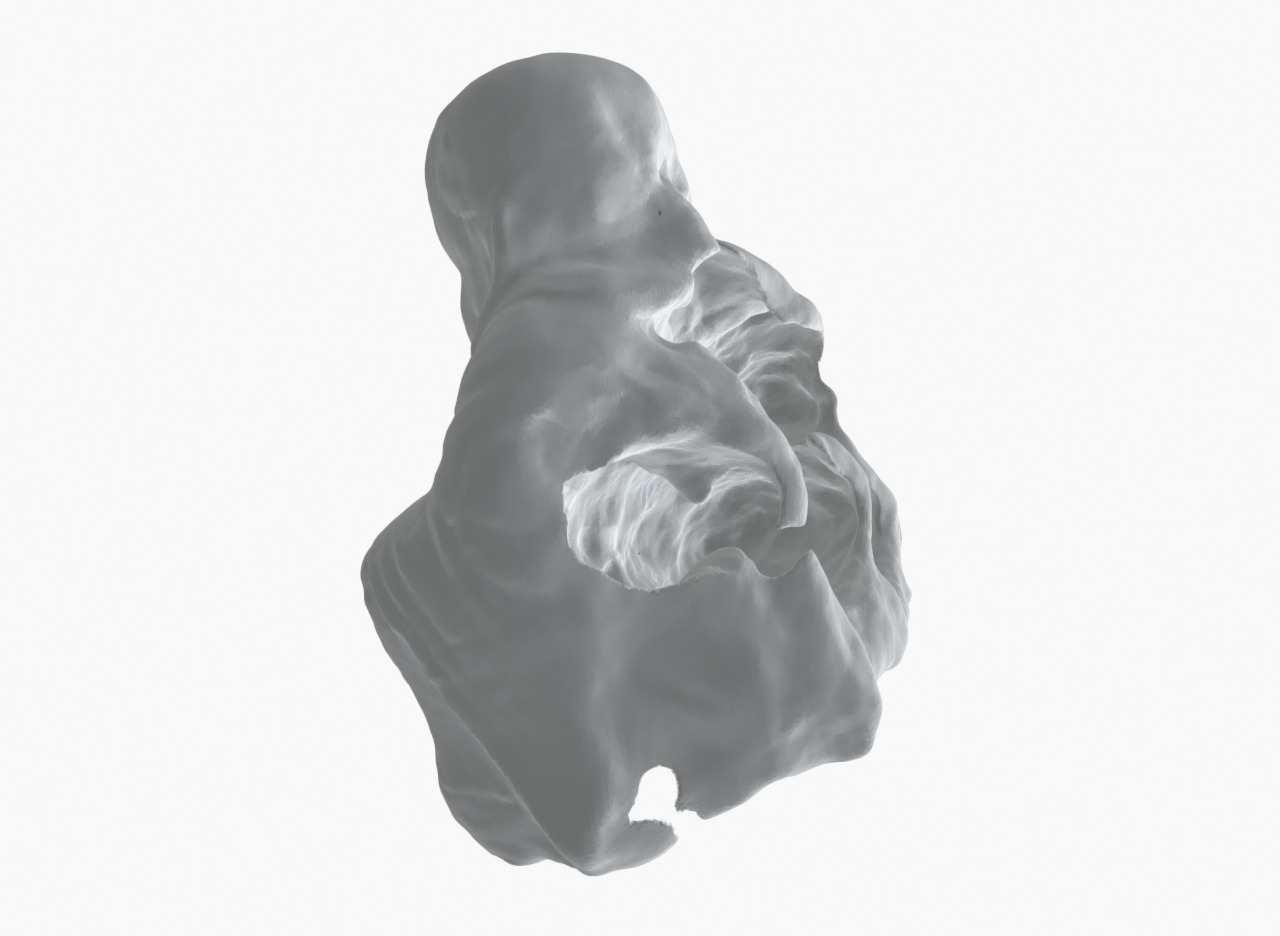
\includegraphics[width=0.2\textwidth]{images/chapter5_img/MeshReconResults/PositionalEncoding/114-HiddenView.jpg} & 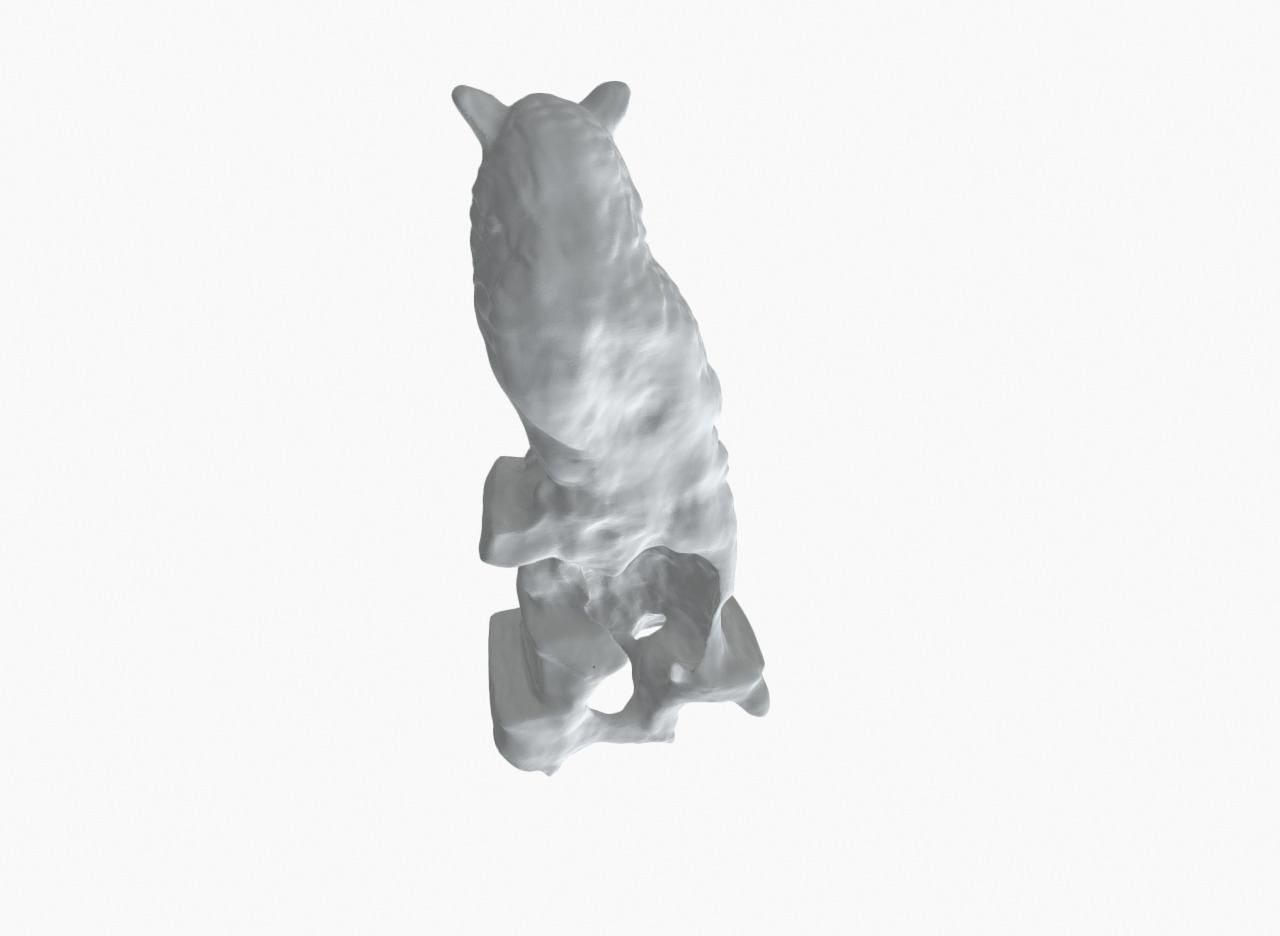
\includegraphics[width=0.2\textwidth]{images/chapter5_img/MeshReconResults/PositionalEncoding/122-HiddenView.jpg} \\
\hline
Stylemod NFFB & 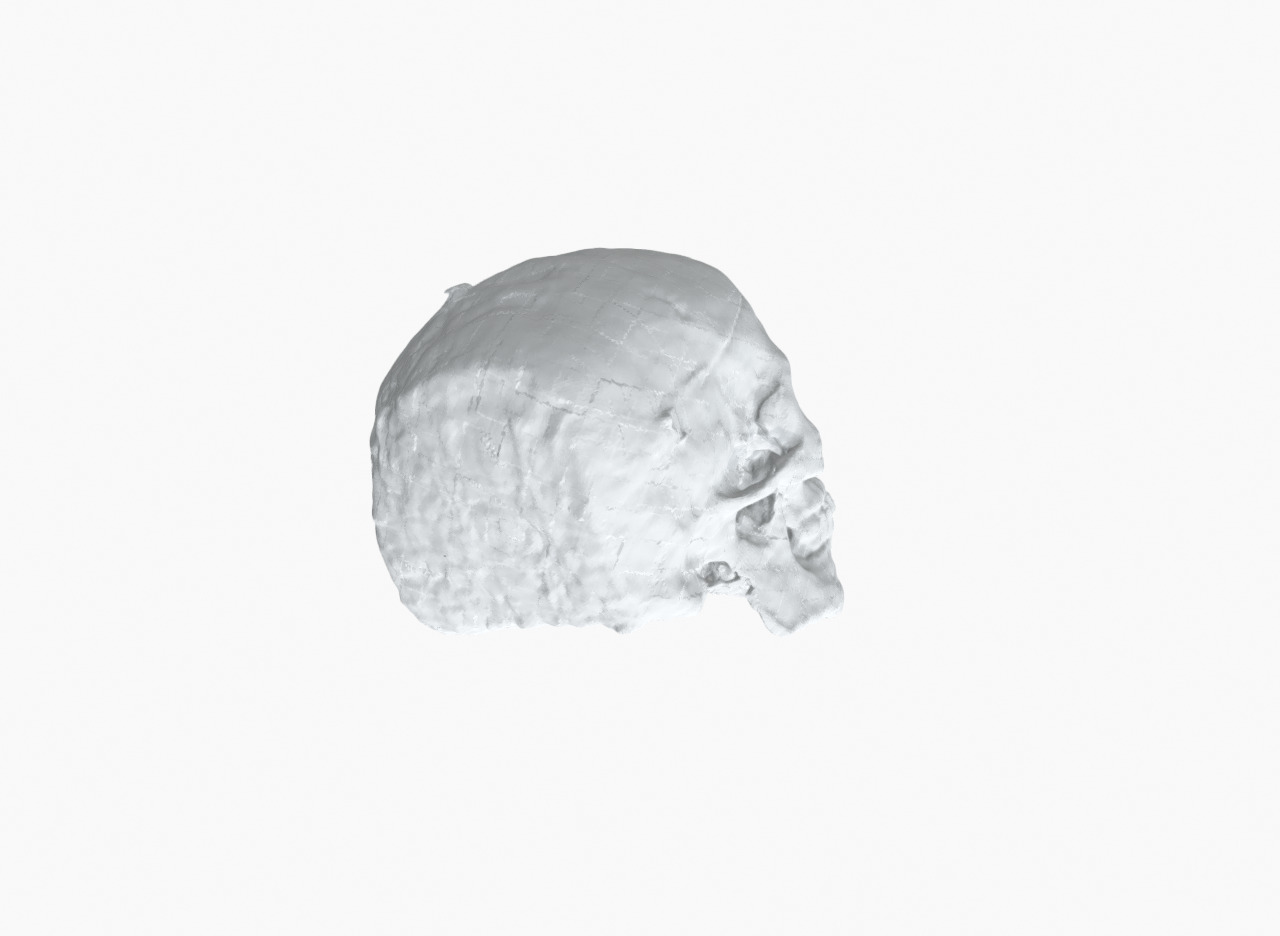
\includegraphics[width=0.2\textwidth]{images/chapter5_img/MeshReconResults/StylemodNFFB/65_HiddenView.jpg} & 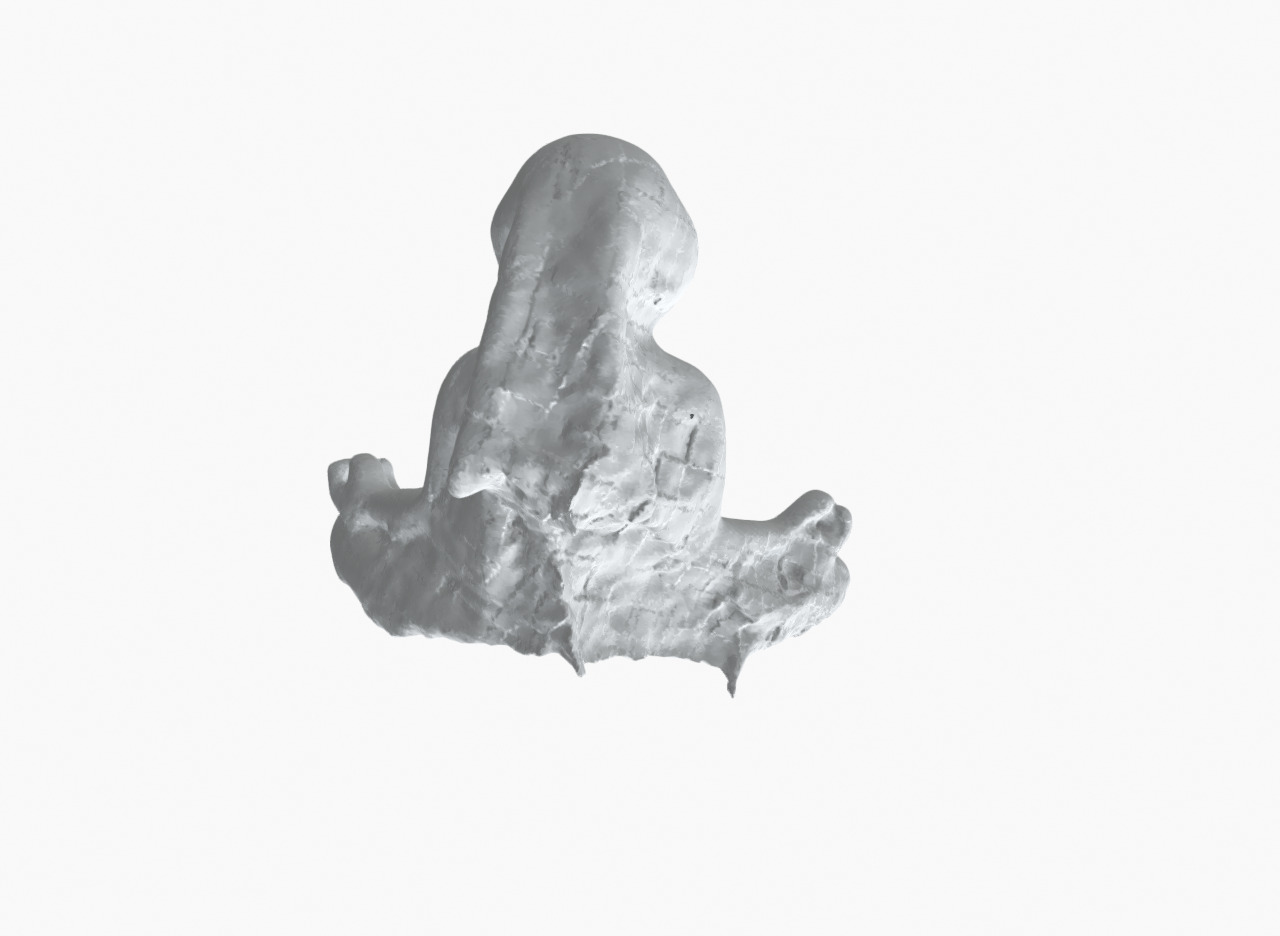
\includegraphics[width=0.2\textwidth]{images/chapter5_img/MeshReconResults/StylemodNFFB/110_HiddenView.jpg} & 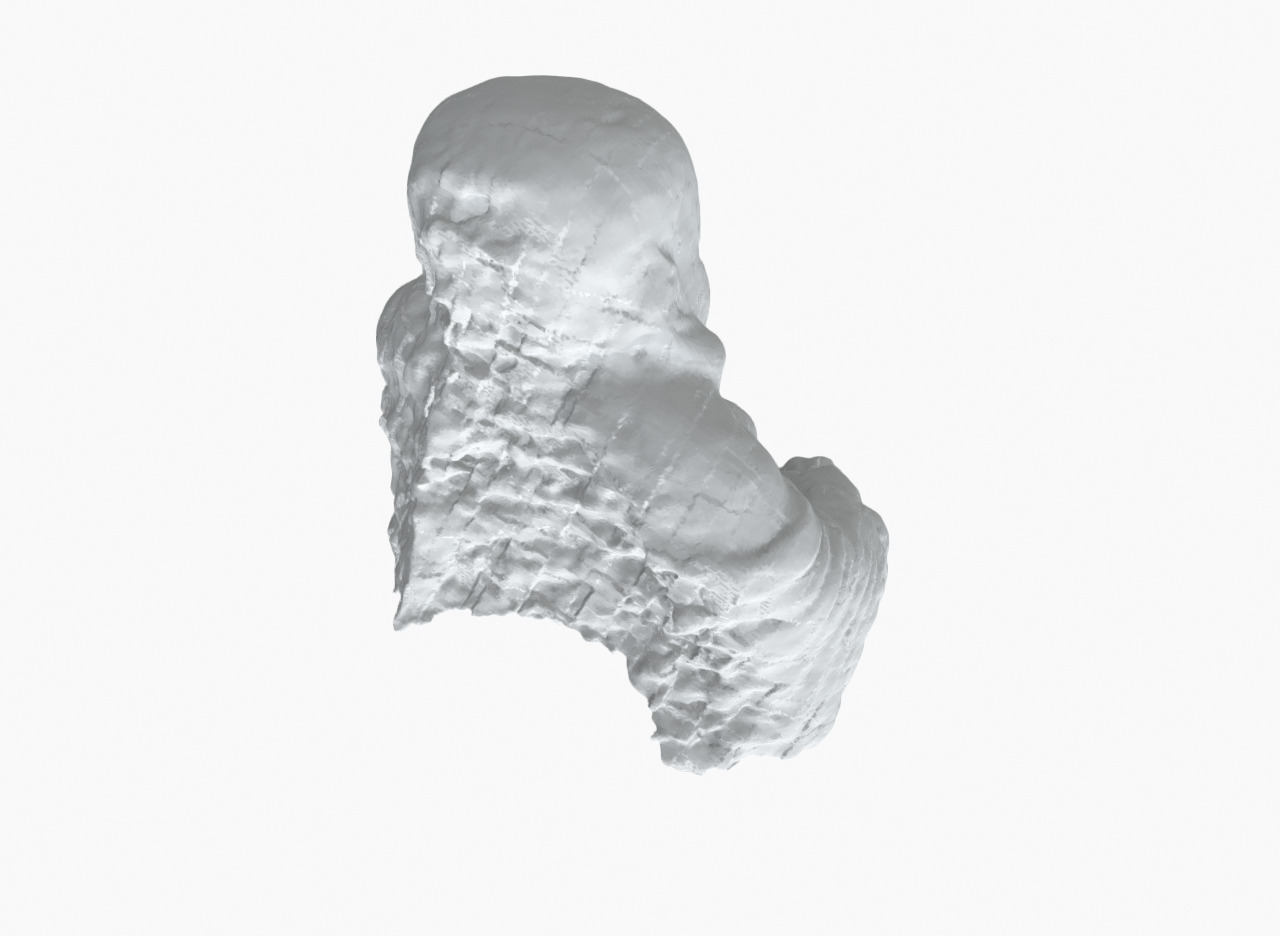
\includegraphics[width=0.2\textwidth]{images/chapter5_img/MeshReconResults/StylemodNFFB/114_HiddenView.jpg} & 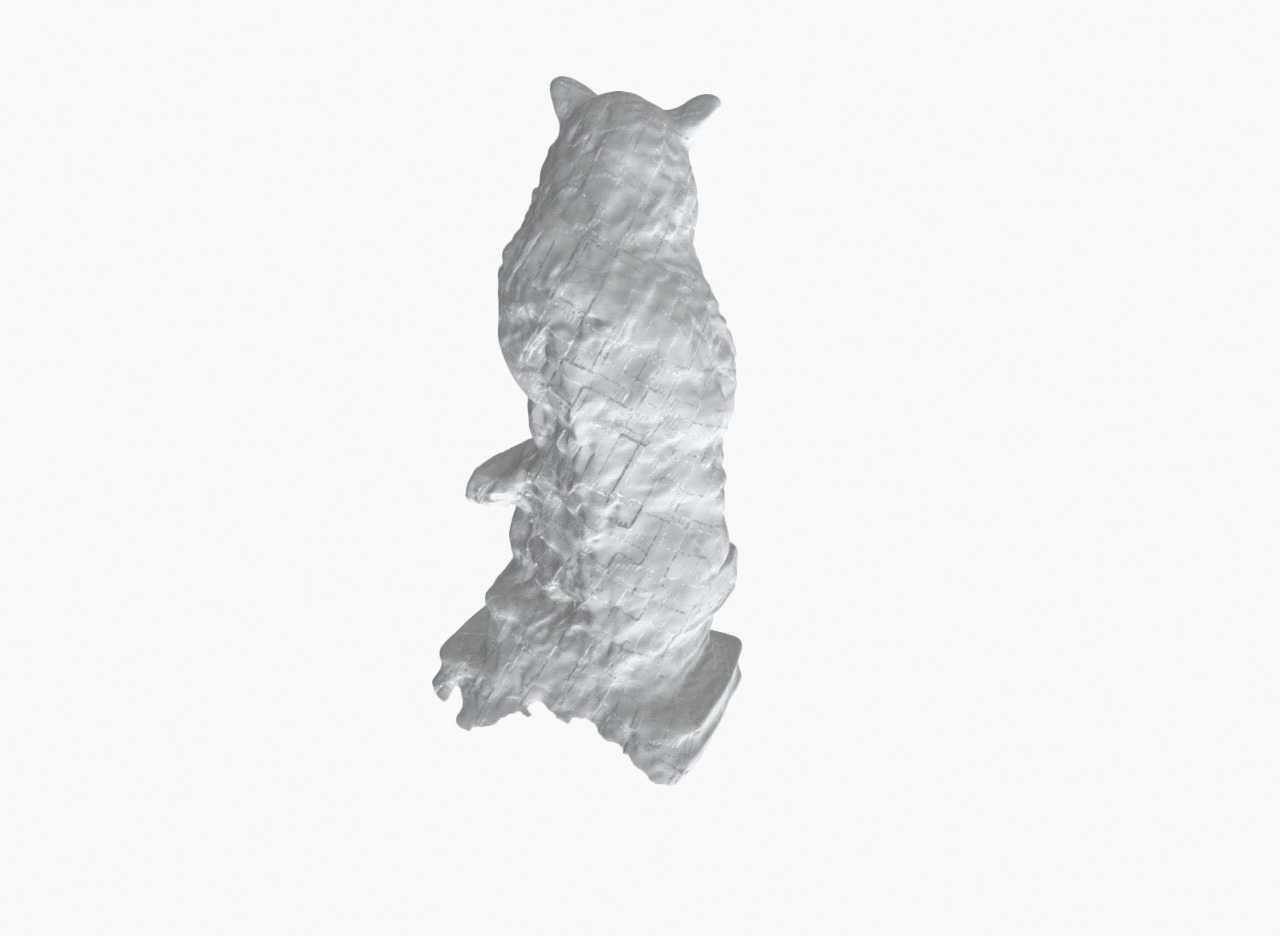
\includegraphics[width=0.2\textwidth]{images/chapter5_img/MeshReconResults/StylemodNFFB/122_HiddenView.jpg} \\
\hline
StylemodNFFB TCNN & 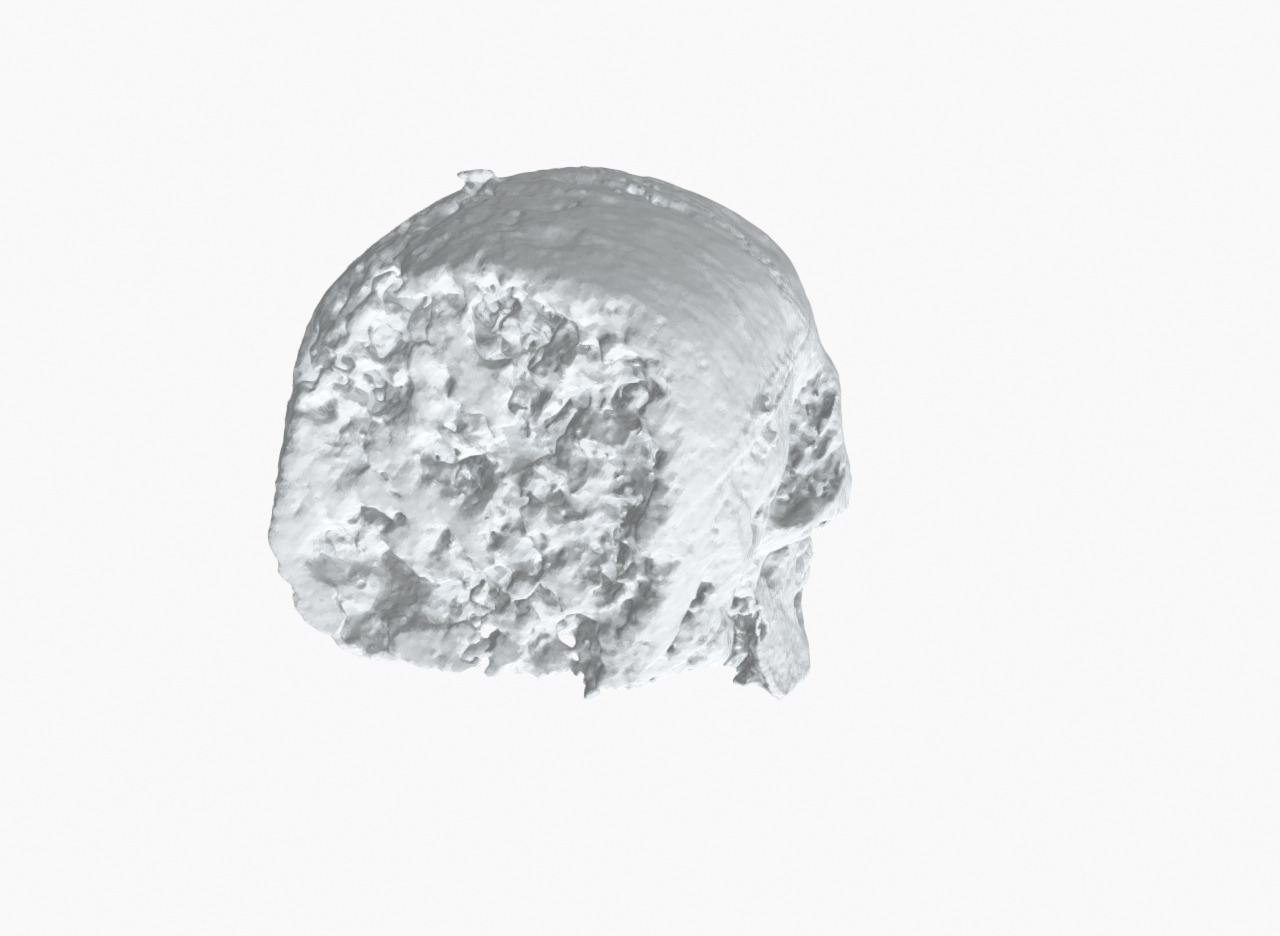
\includegraphics[width=0.2\textwidth]{images/chapter5_img/MeshReconResults/TinyCudaNN-StylemodNFFB/65_2000_HiddenView.jpg} & 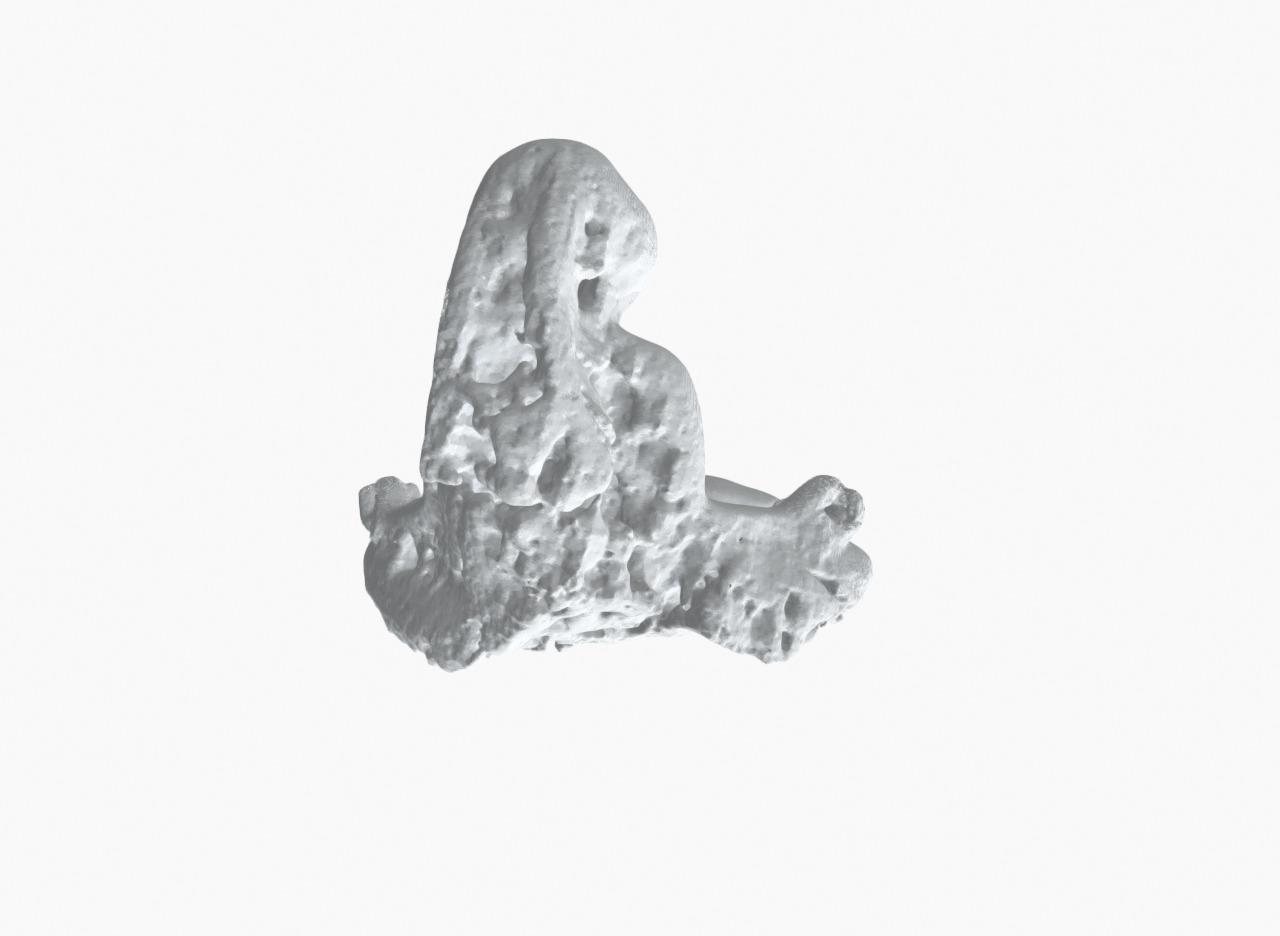
\includegraphics[width=0.2\textwidth]{images/chapter5_img/MeshReconResults/TinyCudaNN-StylemodNFFB/110_bad_HiddenView.jpg} & 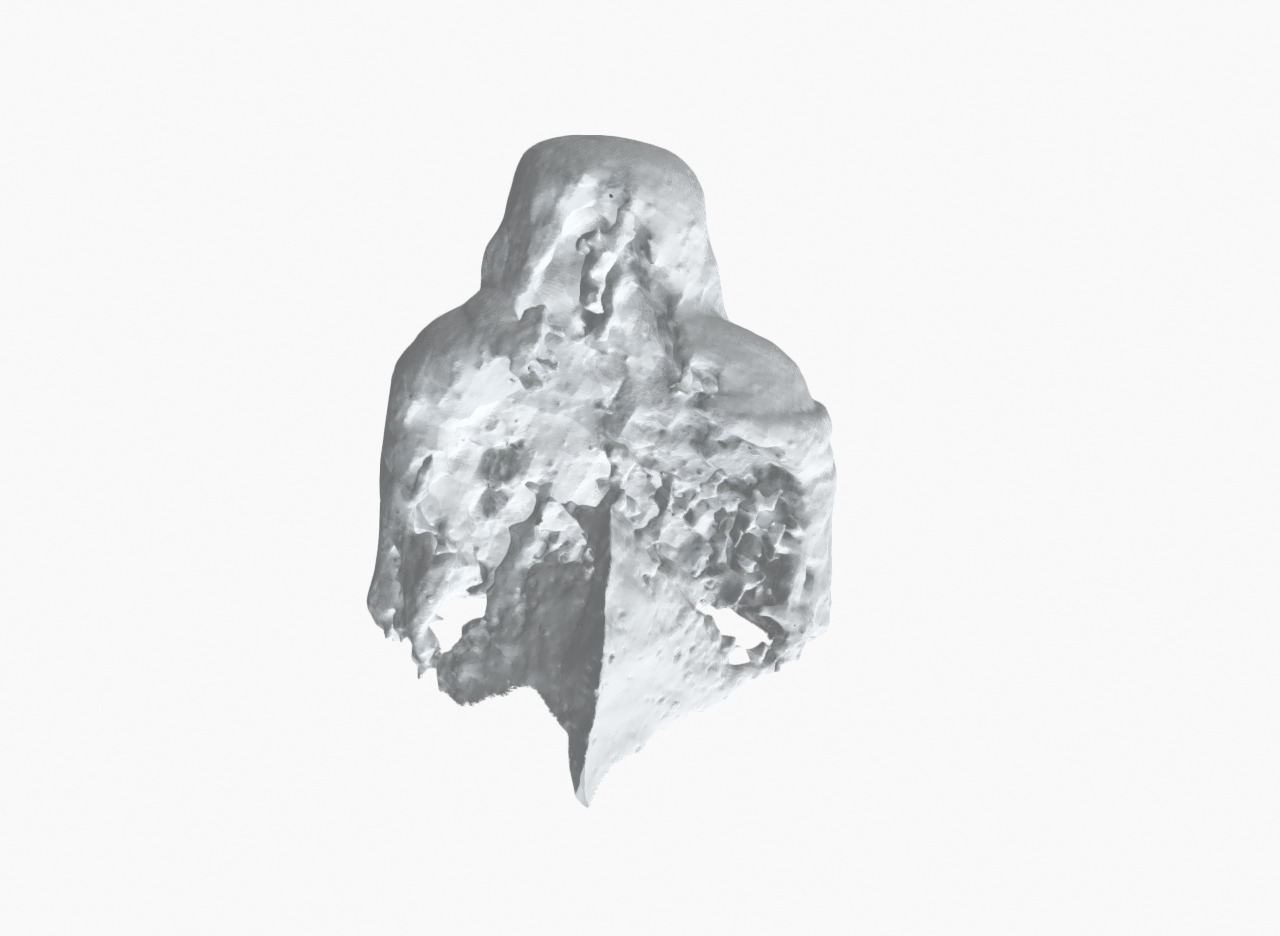
\includegraphics[width=0.2\textwidth]{images/chapter5_img/MeshReconResults/TinyCudaNN-StylemodNFFB/114_2000_HiddenVIew.jpg} & 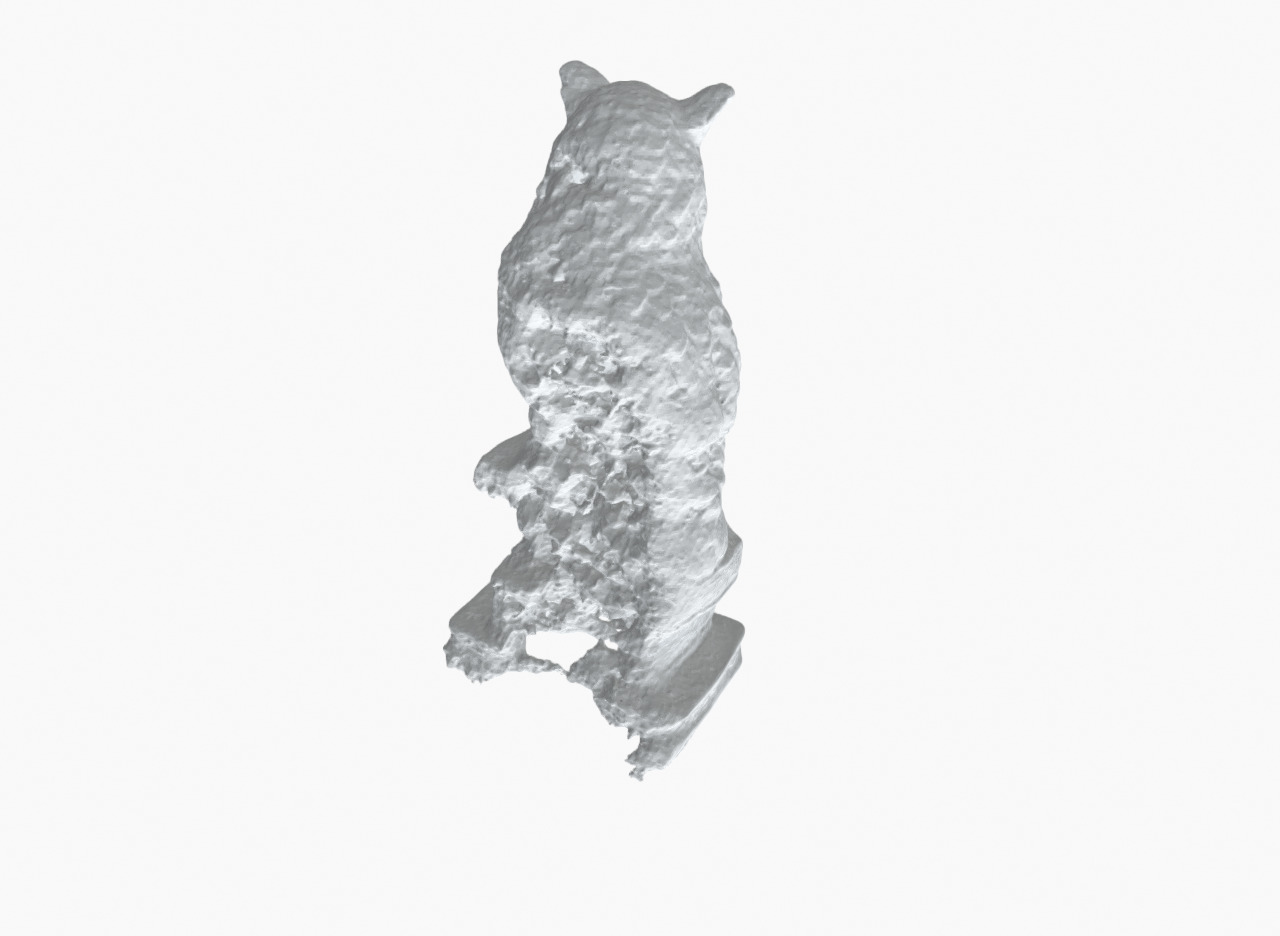
\includegraphics[width=0.2\textwidth]{images/chapter5_img/MeshReconResults/TinyCudaNN-StylemodNFFB/122_HiddenView.jpg} \\
\hline
\end{tabularx}
\caption{Πίνακας Γεωμετρίας Κρυφής Όψης \enit{3D} μοντέλων - Έλεγχος Γενίκευσης}
\end{table}

Τα παραπάνω αποτελούν τις γεωμετρίες που εξάγονται από το πεδίο \enit{SDF} με χρήση του αλγορίθμου \enit{Marching Cubes}. Παρατηρείται, ότι τα δίκτυα υψηλοσυχνοτικής κωδικοποίησης πετυχαίνουν μεγαλύτερη λεπτομέρεια και γενικεύουν καλύτερα στην πίσω όψη που δεν υπάρχουν δεδομένα. Επίσης  καταφέρνουν να αποτυπώσουν περιοχές που παρουσιάζουν μεγάλη μεταβολή της παραγώγου δηλαδή τρύπες στα μοντέλα κάτι το οποίο το IDR χωρίς το δίκτυο κωδικοποίησης δεν μπορεί να μάθει. 

\subsection{Πίνακες Απόστασης Chamfer}
H αξιολόγηση ολοκληρώνεται παρουσιάζοντας την μετρική αξιολόγησης της γεωμετρίας των \enit{3D} μοντέλων. Δίνονται, οι συνολικές αποστάσεις \enit{chamfer} μεταξύ των ανακατασκευασμένων \enit{3D} μοντέλων με τα δεδομένα γεωμετρίας που δίνει το DTU (STL) καθώς και με \enit{3D} μοντέλα που εξάγονται από άλλους αλγορίθμους Multi-Vision Stereo οποίοι θεωρούνται ότι παράγουν αξιόπιστα 3D συμπαγή σχήματα. Ο αλγόριθμος που χρησιμοποιήθηκε βασίζεται στον κώδικα που δίνει το \enit{DTU} για την αξιολόγηση \cite{Jensen14a}. Παρόλα αυτά δεν είναι ο  κώδικα σε Matlab που παρέχεται στο MVS DTU αποθετήριο, αλλά είναι δημοσιευμένος(\href{Htps://github.com/jzhangbs/DTUeval-python}{Htps://github.com/jzhangbs/DTUeval-python}) κώδικας αξιολόγησης γραμμένος  σε python και χρησιμοποιεί την \enit{sklearn} για τα μοντέλα πλησιέστερου γείτονα (s2d, d2s eval data to scan, scan to data). Δημιουργεί το νέφος σημείων εφαρμόζοντας υποδειγματοληψία των συμπαγών δομών και υπολογίζει την απόσταση των γειτόνων μέσω αλγορίθμου δένδρου πλησιέστερων γειτόνων διαμερισμού του χώρου (\enit{kd-tree}). 
\begin{table}[H]
\resizebox{\textwidth}{!}{%
\begin{tabular}{c|cccccccccccccccc|}
\cline{2-17}
 &
  \multicolumn{16}{c|}{Chamfer Distance(mm) ανά scan {[}65, 110, 114, 122{]}} \\ \hline
\multicolumn{1}{|l|}{Μέθοδος Εξαγωγής GT Mesh} &
  \multicolumn{4}{c|}{\begin{tabular}[c]{@{}c@{}}STL\\  DTU scans\end{tabular}} &
  \multicolumn{4}{c|}{\begin{tabular}[c]{@{}c@{}}Camp\\ MVS algorithm\end{tabular}} &
  \multicolumn{4}{c|}{\begin{tabular}[c]{@{}c@{}}Furu\\ MVS algorithm\end{tabular}} &
  \multicolumn{4}{c|}{\begin{tabular}[c]{@{}c@{}}Tola\\ MVS algorithm\end{tabular}} \\ \hline
\multicolumn{1}{|c|}{Positional Encoding} &
  \multicolumn{1}{c|}{0.971} &
  \multicolumn{1}{c|}{\textbf{1.117}} &
  \multicolumn{1}{c|}{0.5} &
  \multicolumn{1}{c|}{0.58} &
  \multicolumn{1}{c|}{1.27} &
  \multicolumn{1}{c|}{\textbf{0.84}} &
  \multicolumn{1}{c|}{0.49} &
  \multicolumn{1}{c|}{0.55} &
  \multicolumn{1}{c|}{1.70} &
  \multicolumn{1}{c|}{\textbf{1.20}} &
  \multicolumn{1}{c|}{0.74} &
  \multicolumn{1}{c|}{0.83} &
  \multicolumn{1}{c|}{2.36} &
  \multicolumn{1}{c|}{\textbf{0.96}} &
  \multicolumn{1}{c|}{0.59} &
  1.02 \\ \hline
\multicolumn{1}{|c|}{MR HashGrid3D} &
  \multicolumn{1}{c|}{1.13} &
  \multicolumn{1}{c|}{1.32} &
  \multicolumn{1}{c|}{0.63} &
  \multicolumn{1}{c|}{0.601} &
  \multicolumn{1}{c|}{1.22} &
  \multicolumn{1}{c|}{0.99} &
  \multicolumn{1}{c|}{0.491} &
  \multicolumn{1}{c|}{\textbf{0.52}} &
  \multicolumn{1}{c|}{1.72} &
  \multicolumn{1}{c|}{1.31} &
  \multicolumn{1}{c|}{0.80} &
  \multicolumn{1}{c|}{0.83} &
  \multicolumn{1}{c|}{\textbf{2.13}} &
  \multicolumn{1}{c|}{1.11} &
  \multicolumn{1}{c|}{0.67} &
  1.03 \\ \hline
\multicolumn{1}{|c|}{NFFB} &
  \multicolumn{1}{c|}{1.00} &
  \multicolumn{1}{c|}{1.36} &
  \multicolumn{1}{c|}{\textbf{0.43}} &
  \multicolumn{1}{c|}{0.58} &
  \multicolumn{1}{c|}{1.29} &
  \multicolumn{1}{c|}{1.05} &
  \multicolumn{1}{c|}{\textbf{0.413}} &
  \multicolumn{1}{c|}{0.523} &
  \multicolumn{1}{c|}{1.75} &
  \multicolumn{1}{c|}{1.34} &
  \multicolumn{1}{c|}{\textbf{0.64}} &
  \multicolumn{1}{c|}{0.81} &
  \multicolumn{1}{c|}{2.24} &
  \multicolumn{1}{c|}{1.15} &
  \multicolumn{1}{c|}{\textbf{0.46}} &
  1.00 \\ \hline
\multicolumn{1}{|c|}{StylemodNFFB} &
  \multicolumn{1}{c|}{\textbf{0.957}} &
  \multicolumn{1}{c|}{1.50} &
  \multicolumn{1}{c|}{0.45} &
  \multicolumn{1}{c|}{\textbf{0.543}} &
  \multicolumn{1}{c|}{\textbf{1.2}} &
  \multicolumn{1}{c|}{1.03} &
  \multicolumn{1}{c|}{0.42} &
  \multicolumn{1}{c|}{\textbf{0.52}} &
  \multicolumn{1}{c|}{\textbf{1.65}} &
  \multicolumn{1}{c|}{1.44} &
  \multicolumn{1}{c|}{0.65} &
  \multicolumn{1}{c|}{\textbf{0.79}} &
  \multicolumn{1}{c|}{2.14} &
  \multicolumn{1}{c|}{1.29} &
  \multicolumn{1}{c|}{0.47} &
  0.99 \\ \hline
\multicolumn{1}{|c|}{StylemodNFFB (TinyCudaNN)} &
  \multicolumn{1}{c|}{1.11} &
  \multicolumn{1}{c|}{2.44} &
  \multicolumn{1}{c|}{1.66} &
  \multicolumn{1}{c|}{0.59} &
  \multicolumn{1}{c|}{1.48} &
  \multicolumn{1}{c|}{2.02} &
  \multicolumn{1}{c|}{1.519} &
  \multicolumn{1}{c|}{0.54} &
  \multicolumn{1}{c|}{1.99} &
  \multicolumn{1}{c|}{2.39} &
  \multicolumn{1}{c|}{1.70} &
  \multicolumn{1}{c|}{0.81} &
  \multicolumn{1}{c|}{2.44} &
  \multicolumn{1}{c|}{2.46} &
  \multicolumn{1}{c|}{1.81} &
  \textbf{0.98} \\ \hline
\end{tabular}%
}

\caption{Πίνακας Μετρικών Μέσης Απόστασης Chamfer}
\end{table}



Παρατηρώντας τον παραπάνω πίνακα, βλέπουμε πως διαφορετικοί αλγόριθμοι είναι πιο καλοί ανά κωδικοποίηση. Κατά πλειοψηφία βέβαια οι καλύτερες ανακατασκευές έχουν γίνει με το \enit{StylemodNFFB}. Η ασυνέπεια που παρατηρείται οφείλεται στο δύσκολο περιεχόμενο φωτισμού των σκηνών 110 και 114 που μπερδεύουν το πεδίο γεωμετρίας. Ταυτόχρονα η εξαγωγή των πλεγμάτων από τις έμμεσες αναπαραστάσεις στο \enit{Positional Encoding} λόγω έγινε με λίγο μεγαλύτερη ανάλυση επομένως έχει μεγαλύτερη λεπτομέρεια χωρίς να είναι απαραίτητα καλύτερη ανακατασκευή.

Πάνω σε αυτό σημαντική σημείωση για τον αναγνώστη είναι πως λόγω περιορισμών μνήμης στη \enit{GPU}(\enit{8Gb Vram}) που χρησιμοποιήθηκε για τα πειράματα, η εξαγωγή των πλεγμάτων από τις έμμεσες αναπαραστάσεις έχει γίνει σε χαμηλή ανάλυση(ανάλυση αλγόριθμου \enit{Marching Cubes} βλ.\ref{section:appendix-algorithms}). Αυτό έχει άμεσο αντίκτυπο στα αποτελέσματα αφού παρέχεται μικρότερο επίπεδο ανάλυσης από ότι δύναται να δοθεί και συνεπώς τα αποτελέσματα της μετρικής \enit{Chamfer} είναι χειρότερα από όσο θα μπορούσαν να είναι. \footnote{η κωδικοποίηση FourierFeatures παραλείπεται γιατί η εξαγωγή των πλεγμάτων έχει γίνει με σημαντικά μεγαλύτερη ανάλυση στην υπολογιστική συστοιχία του ΑΠΘ και τα αποτελέσματα είναι πολύ καλύτερα αλλά δεν μπορούν να συγκριθούν με τα υπόλοιπα.}
\clearpage
\subsubsection{Οπτική Παρουσίαση Chamfer Απόστασης}
Ενδεικτικά δίνεται το οπτικό αποτέλεσμα που παράγει ο αλγόριθμος αξιολόγησης πλεγμάτων για το δίκτυο StylemodNFFB. Το οπτικό αποτέλεσμα που παράγεται είναι και αυτό νέφος σημείων και των δύο σκηνών έτσι δίνεται φωτογραφία. Οι εικόνες είναι 2 μια που δείχνει την απόσταση των παραγόμενων δεδομένων από το τρισδιάστατο scan(d2s) και μια το ανάποδο(s2d). 



\begin{figure}[H]
  \begin{minipage}{0.5\linewidth}
    \centering
    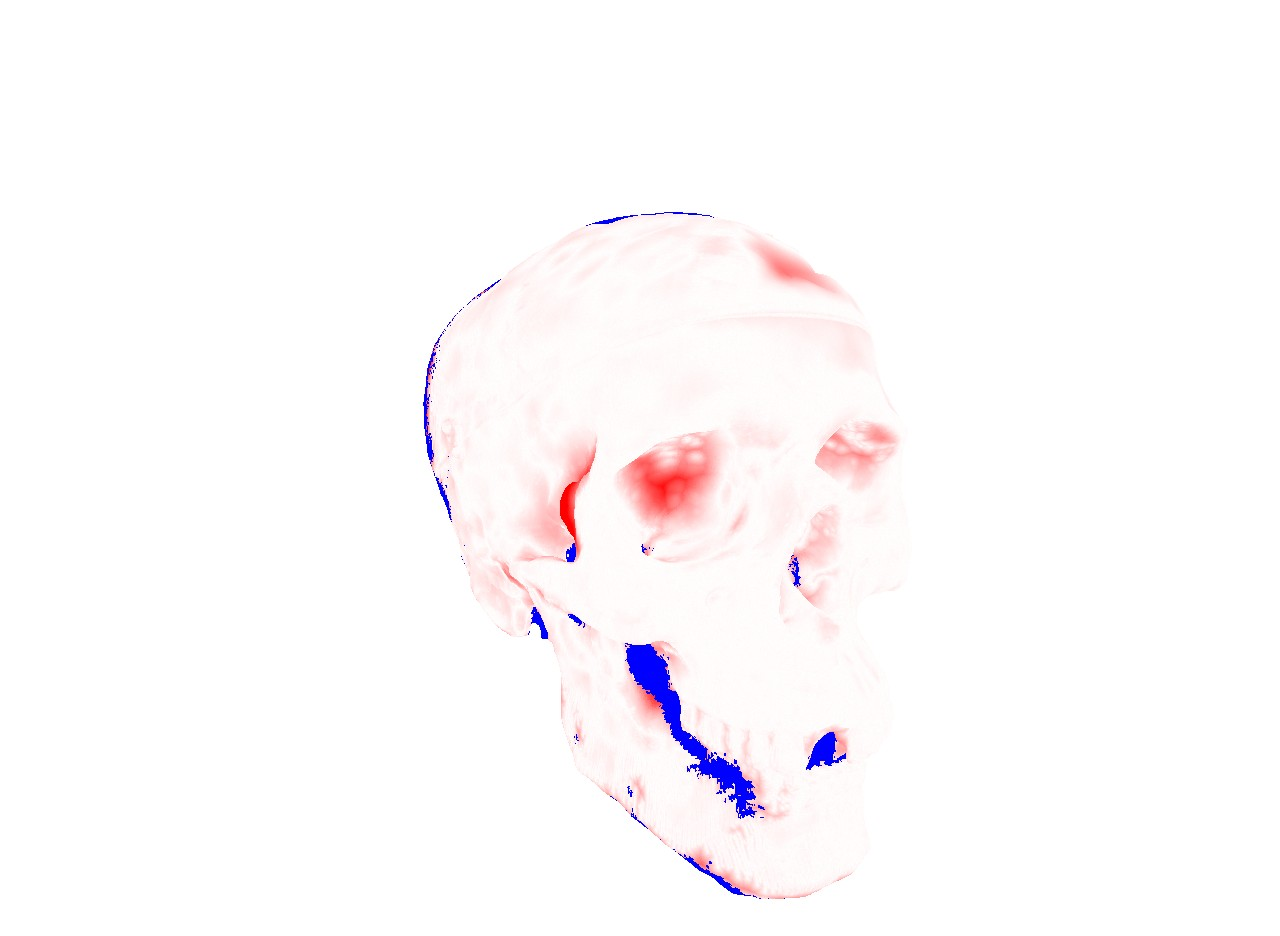
\includegraphics[width=\linewidth]{images/chapter5_img/ChamferDistViz/d2s_stylemod_nffb_front.jpg}
    \subcaption{d2s front}
  \end{minipage}%
  \begin{minipage}{0.5\linewidth}
    \centering
    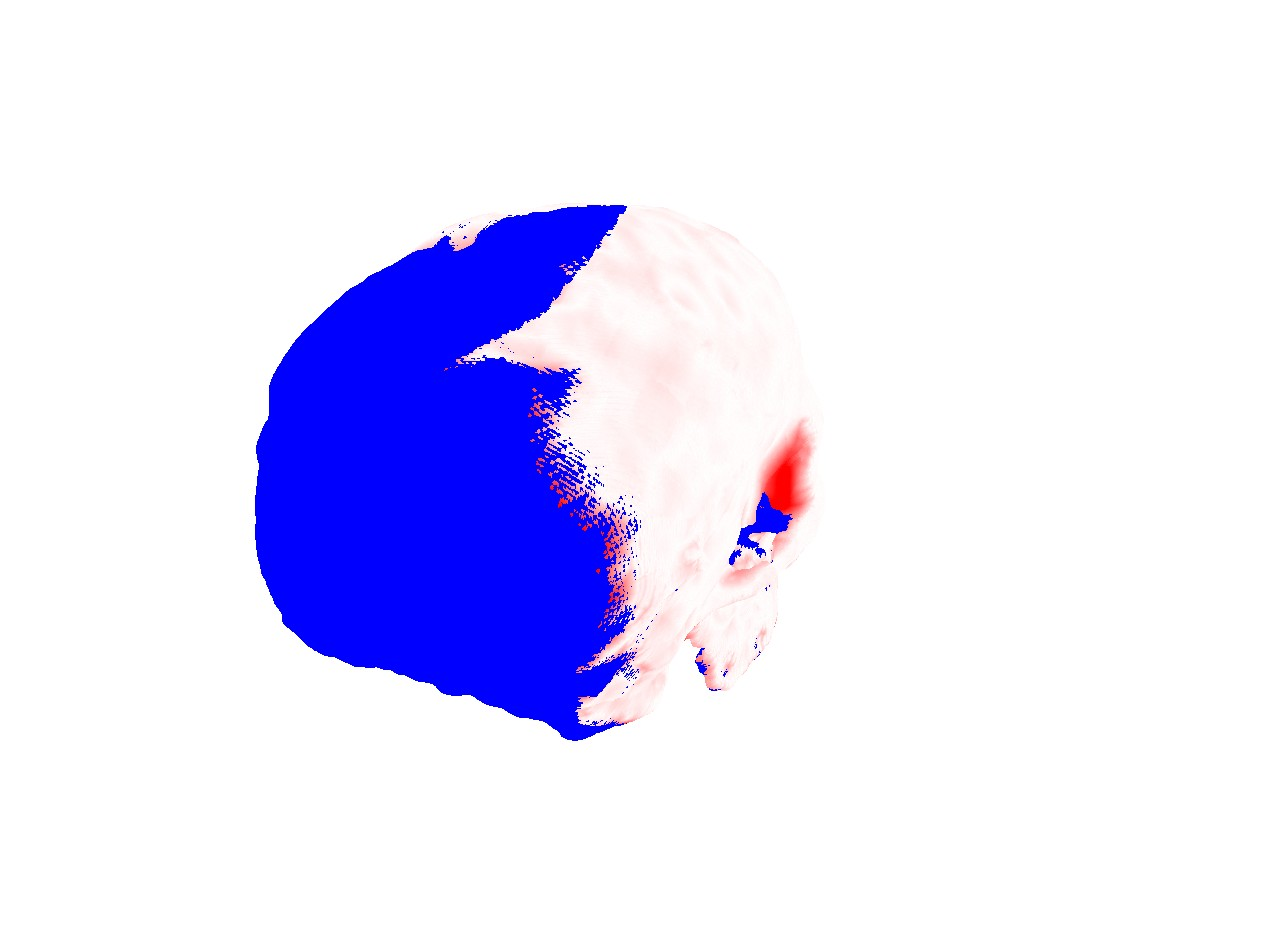
\includegraphics[width=\linewidth]{images/chapter5_img/ChamferDistViz/d2s_skull_stylemodnffb_back.jpg}
    \subcaption{d2s back}
  \end{minipage}
  \begin{minipage}{0.5\linewidth}
    \centering
    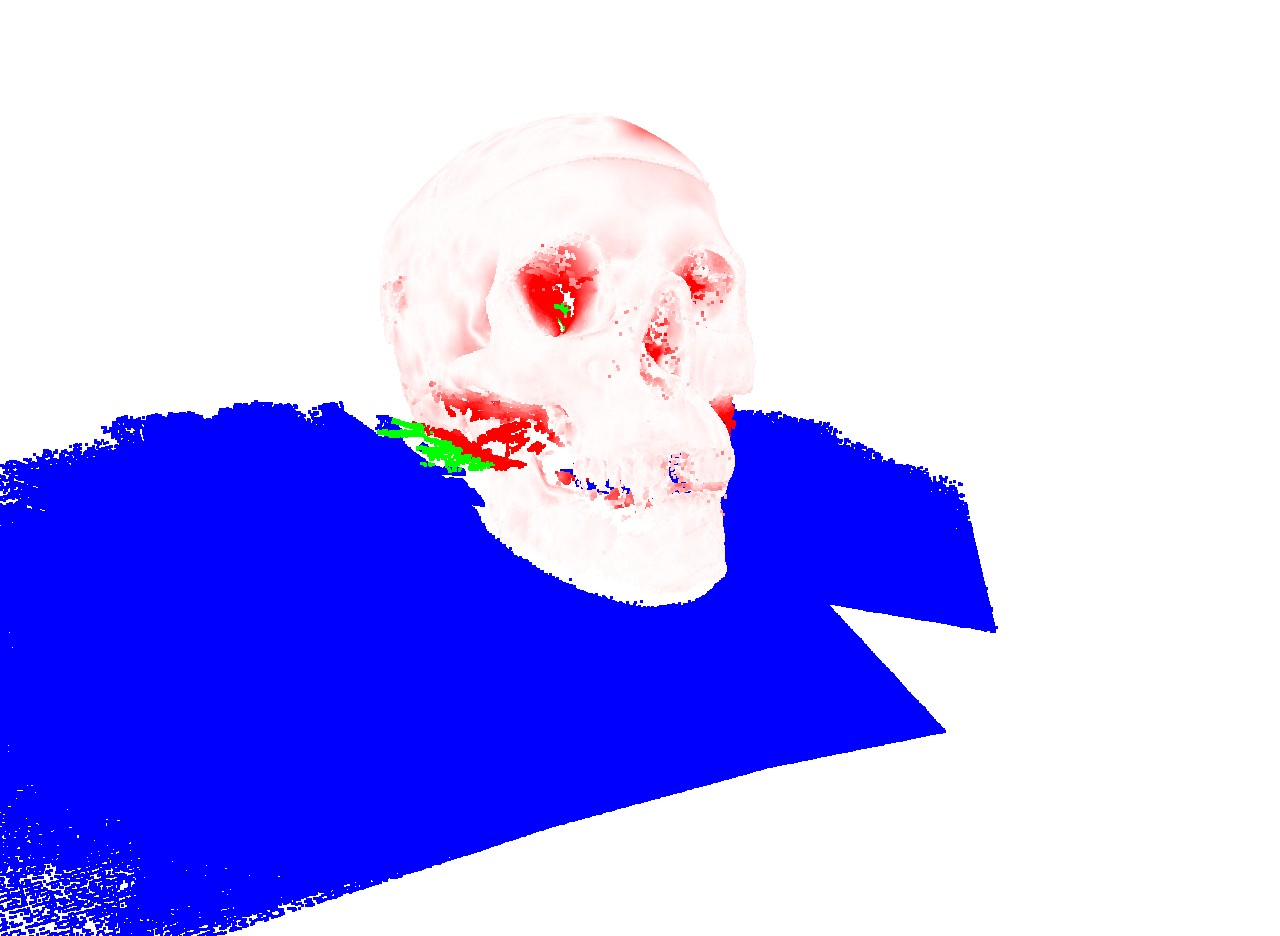
\includegraphics[width=\linewidth]{images/chapter5_img/ChamferDistViz/s2d_stylemodnffb_64_front.jpg}
    \subcaption{s2d front}
  \end{minipage}%
  \begin{minipage}{0.5\linewidth}
    \centering
    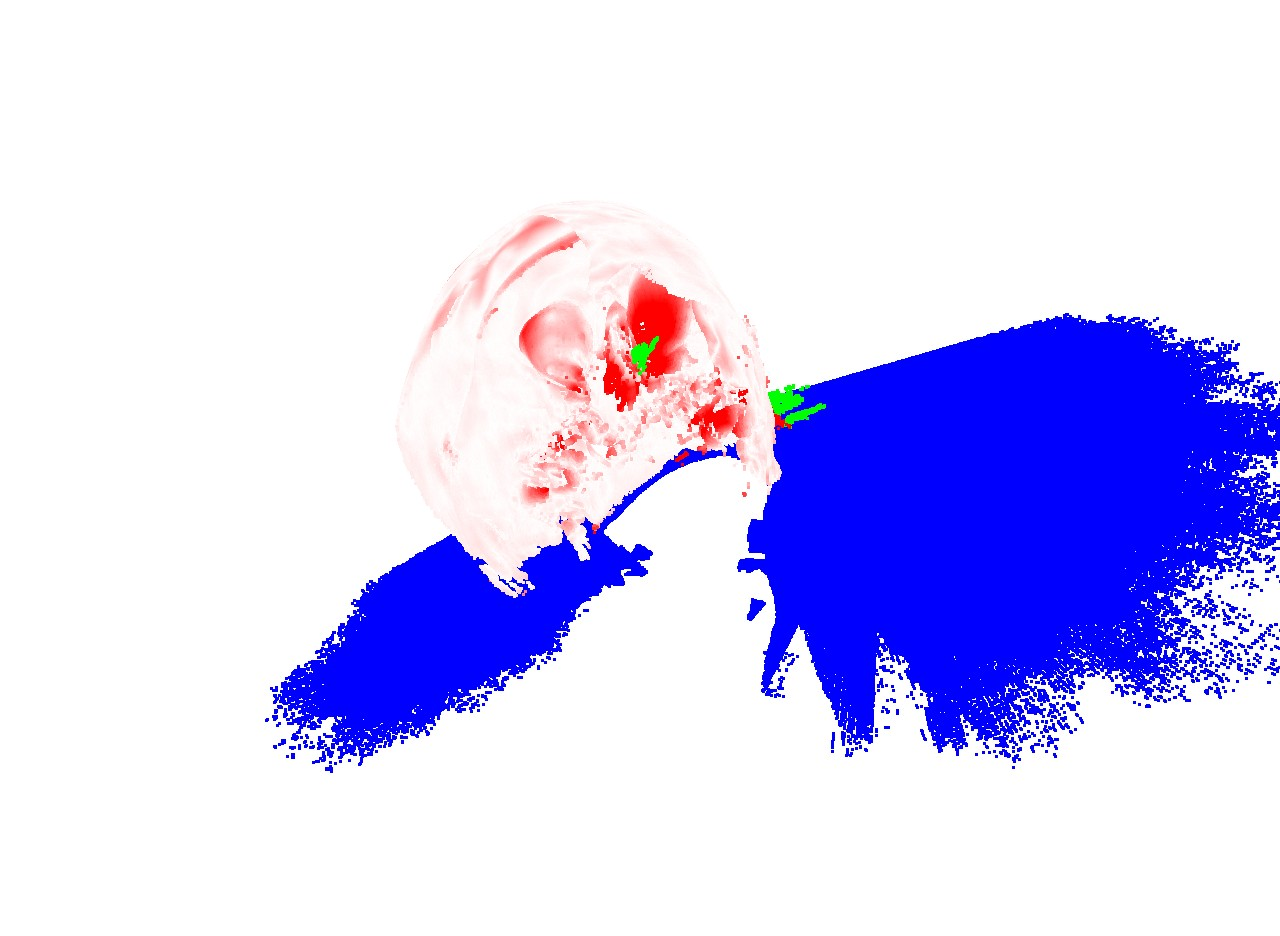
\includegraphics[width=\linewidth]{images/chapter5_img/ChamferDistViz/s2d_stylemodnffb_65_back.jpg}
    \subcaption{s2d back}
  \end{minipage}
  \caption{Οπτική αποτύπωση Chamfer απόστασης}
\end{figure}

Τα κόκκινα σημεία είναι μικρές αποστάσεις στα όρια του στατιστικού λάθους. Τα μπλε σημεία είναι σημεία που αποτυπώνει η ανακατασκευή, ενώ δεν έχει το point cloud της σάρωσης στην  d2s περίπτωση. Αντίθετα στην άλλη περίπτωση s2d είναι σημεία που σαρώνονται του αντικειμένου από τις  κλασσικές μεθόδους σάρωσης και δεν μας ενδιαφέρουν. Τέλος τα πράσινα σημεία είναι σημεία που απέχουν μεταξύ ανακατασκευής και σάρωσης τα οποία λανθασμένα βγάζουν οι κλασσικές μέθοδοι σάρωσης MVS.